%%% Hlavní soubor. Zde se definují základní parametry a odkazuje se na ostatní části. %%%

%% Verze pro jednostranný tisk:
% Okraje: levý 40mm, pravý 25mm, horní a dolní 25mm
% (ale pozor, LaTeX si sám přidává 1in)
\documentclass[12pt,a4paper]{report}
\setlength\textwidth{145mm}
\setlength\textheight{247mm}
\setlength\oddsidemargin{15mm}
\setlength\evensidemargin{15mm}
\setlength\topmargin{0mm}
\setlength\headsep{0mm}
\setlength\headheight{0mm}

%% Pokud používáte csLaTeX (doporučeno):
\usepackage{czech}

%% Použité kódování znaků: obvykle latin2, cp1250 nebo utf8:
\usepackage[utf8]{inputenc}

%% Ostatní balíčky
\usepackage{graphicx}
\usepackage{amsthm}

%% Balíček hyperref, kterým jdou vyrábět klikací odkazy v PDF,
%% ale hlavně ho používáme k uložení metadat do PDF (včetně obsahu).
%% POZOR, nezapomeňte vyplnit jméno práce a autora.
\usepackage[ps2pdf,unicode]{hyperref}   % Musí být za všemi ostatními balíčky
\hypersetup{pdftitle=Webová čtečka a knihovna článků}
\hypersetup{pdfauthor=Adam Juraszek}

\usepackage{framed}
\usepackage{xcolor}

\newlength{\leftbarwidth}
\setlength{\leftbarwidth}{3pt}
\newlength{\leftbarsep}
\setlength{\leftbarsep}{10pt}

\newcommand*{\leftbarcolorcmd}{\color{leftbarcolor}}% as a command to be more flexible
\colorlet{leftbarcolor}{black}

\renewenvironment{leftbar}{%
    \def\FrameCommand{{\leftbarcolorcmd{\vrule width \leftbarwidth\relax\hspace {\leftbarsep}}}}%
    \MakeFramed {\advance \hsize -\width \FrameRestore }%
}{%
    \endMakeFramed
}

%\usepackage{paralist}

%\usepackage{subcaption}

%\usepackage{multirow}

%\usepackage{cancel}

\usepackage{breakurl}
%\usepackage{url}

\usepackage{tabu}

%\usepackage{pdflscape}

%\usepackage{threeparttable}

\usepackage{rotating}

\usepackage[stable]{footmisc}

\usepackage[intoc]{nomencl}
\makenomenclature

\usepackage{xparse}

%~-
\NewDocumentCommand\zkratka{ s o m m }{% s = star, m = mandatory arg
%~+
	\IfBooleanTF{#1}{% with star
	}{% without star
		{\IfNoValueTF{#2}%
			{#3}{#2}}\footnote{#4}%
	}%
	\nomenclature{#3}{#4}%
}%

%~-
\NewDocumentCommand\pojem{ s o m m }{% s = star, m = mandatory arg
%~+
	\IfBooleanTF{#1}{% with star
	}{% without star
		{\IfNoValueTF{#2}%
			{#3}{#2}}\footnote{#4}%
	}%
	\nomenclature{#3}{#4}%
}%

\def\chaptert#1{
	\chapter*{#1}
	\addcontentsline{toc}{chapter}{#1}
}
\def\sectiont#1{
	\section*{#1}
	\addcontentsline{toc}{section}{#1}
}
\def\subsectiont#1{
	\subsection*{#1}
	\addcontentsline{toc}{subsection}{#1}
}

%%% Drobné úpravy stylu

% Tato makra přesvědčují mírně ošklivým trikem LaTeX, aby hlavičky kapitol
% sázel příčetněji a nevynechával nad nimi spoustu místa. Směle ignorujte.
\makeatletter
\def\@makechapterhead#1{
  {\parindent \z@ \raggedright \normalfont
   \Huge\bfseries \thechapter. #1
   \par\nobreak
   \vskip 20\p@
}}
\def\@makeschapterhead#1{
  {\parindent \z@ \raggedright \normalfont
   \Huge\bfseries #1
   \par\nobreak
   \vskip 20\p@
}}
\makeatother

% Toto makro definuje kapitolu, která není očíslovaná, ale je uvedena v obsahu.
\def\chapwithtoc#1{
\chapter*{#1}
\addcontentsline{toc}{chapter}{#1}
}

% Trochu volnější nastavení dělení slov, než je default.
\lefthyphenmin=2
\righthyphenmin=2

\hyphenpenalty=750

\begin{document}

%%% Titulní strana práce

\pagestyle{empty}
\begin{center}

\large

Univerzita Karlova v Praze

\medskip

Matematicko-fyzikální fakulta

\vfill

{\bf\Large BAKALÁŘSKÁ PRÁCE}

\vfill

\centerline{\mbox{
\includegraphics[width=60mm]{img/logo.eps}}}

\vfill
\vspace{5mm}

{\LARGE Adam Juraszek}

\vspace{15mm}

% Název práce přesně podle zadání
{\LARGE\bfseries Webová čtečka a knihovna článků}

\vfill

% Název katedry nebo ústavu, kde byla práce oficiálně zadána
% (dle Organizační struktury MFF UK)
Katedra softwarového inženýrství

\vfill

\begin{tabular}{rl}

Vedoucí bakalářské práce: & Mgr. Martin Svoboda \\
\noalign{\vspace{2mm}}
Studijní program: & Informatika \\
\noalign{\vspace{2mm}}
Studijní obor: & obecná informatika \\
\end{tabular}

\vfill

% Zde doplňte rok
Praha 2013

\end{center}


%%% Následuje vevázaný list -- kopie podepsaného "Zadání bakalářské práce".
%%% Toto zadání NENÍ součástí elektronické verze práce, nescanovat.

%%% Na tomto místě mohou být napsána případná poděkování (vedoucímu práce,
%%% konzultantovi, tomu, kdo zapůjčil software, literaturu apod.)

\noindent
Poděkování. % TODO podekovani


%%% Strana s čestným prohlášením k bakalářské práci

\newpage

\vglue 0pt plus 1fill

\noindent
Prohlašuji, že jsem tuto bakalářskou práci vypracoval(a) samostatně a výhradně
s~použitím citovaných pramenů, literatury a dalších odborných zdrojů.

\medskip\noindent
Beru na~vědomí, že se na moji práci vztahují práva a povinnosti vyplývající
ze zákona č. 121/2000 Sb., autorského zákona v~platném znění, zejména skutečnost,
že Univerzita Karlova v Praze má právo na~uzavření licenční smlouvy o~užití této
práce jako školního díla podle §60 odst. 1 autorského zákona.

\vspace{10mm}

\hbox{\hbox to 0.5\hsize{%
V ........ dne ............
\hss}\hbox to 0.5\hsize{%
Podpis autora
\hss}}

\vspace{20mm}
\newpage

%%% Povinná informační strana bakalářské práce

\vbox to 0.5\vsize{
\setlength\parindent{0mm}
\setlength\parskip{5mm}

Název práce:
Webová čtečka a knihovna článků
% přesně dle zadání

Autor: % jméno
Adam Juraszek

Katedra:  % Případně Ústav:
Katedra softwarového inženýrství
% dle Organizační struktury MFF UK

Vedoucí bakalářské práce:
RNDr. Martin Svoboda, Katedra softwarového inženýrství
% dle Organizační struktury MFF UK, případně plný název pracoviště mimo MFF UK

Abstrakt: % TODO abstract
% abstrakt v rozsahu 80-200 slov; nejedná se však o opis zadání bakalářské práce

Klíčová slova: % TODO klicova slova
% 3 až 5 klíčových slov

\vss}\nobreak\vbox to 0.49\vsize{
\setlength\parindent{0mm}
\setlength\parskip{5mm}

Title: % TODO nazev
% přesný překlad názvu práce v angličtině

Author:
Adam Juraszek

Department: % katedra
Department of Software Engineering
% dle Organizační struktury MFF UK v angličtině


Supervisor: % vedouci
RNDr. Martin Svoboda, Department of Software Engineering
% dle Organizační struktury MFF UK, případně plný název pracoviště
% mimo MFF UK v angličtině

Abstract: % TODO abstract
% abstrakt v rozsahu 80-200 slov v angličtině; nejedná se však o překlad
% zadání bakalářské práce

Keywords: % TODO klicova slova
% 3 až 5 klíčových slov v angličtině

\vss}



%%% Strana s automaticky generovaným obsahem bakalářské práce. U matematických
%%% prací je přípustné, aby seznam tabulek a zkratek, existují-li, byl umístěn
%%% na začátku práce, místo na jejím konci.

\pagestyle{plain}
\setcounter{page}{1}
\tableofcontents



\chaptert{Úvod}

Naše bakalářská práce se zabývá vývojem aplikace -- webové čtečky určené pro náročnější uživatele.
Kromě samozřejmé funkcionality, sledování nejrůznějších RSS kanálů, bude v sobě integrovat i několik dalších služeb, které jsou dle našeho názoru čtečkám blízké.
Myslíme si, že sjednocením vznikne celek, který bude plnit svoji úlohu lépe, než každá ze služeb odděleně.

\sectiont{Historie projektu}

Jelikož je tato práce silně inspirovaná naší zkušeností s dnes již neexistující čtečkou \href{http://www.google.com/reader/about/}{Google Reader}, popíšeme v této části alespoň stručně její historii, osud a náš vztah k ní.

\subsectiont{Používání Google Readeru}

V roce 2005 přišla společnost Google se svojí čtečkou Google Reader.
O několik let později, když jsme tuto čtečku začali používat, jsme byli s jejími možnostmi spokojení a dlouhou dobu pokrývala veškeré naše potřeby.

V roce 2011 byl nahrazen vnitřní mechanismus sdílení položek napojením na sociální síť Google+ od stejné společnosti.
Tento krok z hlediska společnosti Google dává dobrý smysl.
Propagují svoji sociální síť mezi uživateli čtečky a naopak, usnadňují používání čtečky uživatelům sociální sítě.

Z osobních důvodů ale sociální síť Google+ nechceme používat.
Důsledek změny způsobu sdílení položek se nás tedy citelně dotkl a omezil nám možnosti užití této čtečky.

Během dlouhé doby používání čtečky jsme si vypěstovali různé návyky, které nám práci s ní zefektivnily.
Bohužel jsme také narazili na její možnosti; některé operace nešlo provést dostatečně pohodlně a proto jsme je nepoužívali.
Příkladem může být funkcionalita štítků, čtečka je sice nabízela, ale k jejich přiřazení bylo nutné vypsat celý jejich název.
Pro nás to bylo daleko od ideálu: možnost nastavit štítkům klávesové zkratky a přiřazovat je stiskem jediné klávesy.

Stiskem klávesy \verb|"s"| bylo možné položce přidat či odebrat hvězdičku a klávesou \verb|"l"| bylo možné si položku oblíbit.
Nebylo možné přejít na seznam oblíbených položek klávesovou zkratkou, což tento mechanismus pro nás učinilo nepoužitelným.
Oblíbené položky byly úplně zrušeny po změně sdílení na Google+.

Způsob práce se čtečkou v posledním stádiu probíhal následovně.
Přepnuli jsme se na seznam všech položek, procházeli jej lineárně a těm položkám, které nás zaujaly, jsme přiřadili hvězdičku.
Pak jsme se přepnuli na seznam položek s hvězdičkou a procházeli je v náhodném pořadí (podle aktuální nálady).
Jednotlivé články jsme postupně četli a přečteným jsme odebrali hvězdičku.
Některé články nám v tomto seznamu vydržely dlouhé měsíce, jiné jsme vyřadili po několika málo minutách.
Nepoužívali jsme žádný mechanismus, který by umožňoval ukládat položky trvale.

\subsectiont{Konec Google Readeru}

V březnu roku 2013 společnost Google vydala prohlášení, že některé služby budou za nedlouho ukončeny.
Seznam obsahoval i oblíbenou čtečku Google Reader; její provoz bude zrušen k 1. červenci 2013~\cite{google-reader-down}.

Po tomto prohlášení začaly vznikat petice dovolávající se zachování čtečky; přestože získaly tisíce podpisů, osud čtečky nezměnily.
Zároveň začaly zaplavovat internet články obsahující seznam alternativ ke Google Readeru, služeb, ke kterým se mohou aktuální uživatelé uchýlit.

Čtečku Google Reader jsme používali do samého jejího konce.
Nechť odpočívá v pokoji.

\subsectiont{Vznik projektu}

V roce 2012, krátce po změně mechanismu sdílení, jsme zaznamenali vznik projektu \href{http://hiveminedblog.tumblr.com/}{Hivemined}.
Založil ho bývalý uživatel Google Readeru \href{mailto:apodysophilia@gmail.com}{Francis Cleary}; jeho cílem bylo vyvinout náhradu původního Google Readeru.
Postup jeho práce na této náhradě jsme sledovali, nicméně v lednu roku 2012 se odmlčel a nebylo jasné, jestli vývoj dále pokračuje či své snahy zanechal.
Na svém blogu se znovu ozval v listopadu 2012; vývoji čtečky se aktivně věnuje.
Během následujícího půlroku, těsně před uzavřením naší práce, se mu podařilo čtečku dokončit pod názvem \href{http://hivereader.com/}{Hive}.
Poslal nám e-mailem pozvánku k uzavřenému beta testování, bohužel jsme zatím neměli čas čtečku vyzkoušet a zhodnotit.

Během jeho odmlky jsme si vybrali téma bakalářské práce, u kterého jsme se zpočátku částečně inspirovali zmíněným projektem.
Zaměřili jsme se na provázání několika služeb, které dle našeho názoru umožní efektivněji používat rozšířené funkcionality čtečky.
Vycházeli jsme především ze zkušeností s několikaletým používám čtečky od Googlu.
Chtěli jsme zachovat/rozšířit její dobré vlastnosti a naopak se vyvarovat těch, které nepovažujeme za šťastně řešené.
Vzhledem k tomu, že naši aplikaci budeme sami používat, navrhli jsme ji především tak, aby nám vyhovovala.

\sectiont{Členění práce}

V tomto textu se snažíme popsat většinu aspektů aplikace, kterou jsme navrhli a vytvořili.
Aplikaci postupně rozebíráme z několika hledisek.

Nejprve v první kapitole rozčleníme čtečky podle několika kritérií, uvedeme vybrané čtečky a porovnáme je v přehledové tabulce.
Druhou kapitolu věnujeme vymezení problému, kterým se budeme dále zabývat, a jeho popisu.
Ve třetí kapitole představíme existující algoritmy doporučování a zvolíme takový, který bude v našem případě nejvhodnější.
Následující, čtvrtou kapitolu zasvětíme představení technologií a knihoven, jež při implementaci využijeme.

Vlastní návrh aplikace podrobně rozebereme v páté kapitole: její členění z pohledu architektury, s jakými entitami pracuje a jaké procesy v ní probíhají.
V šesté kapitole přiblížíme vlastní fungování aplikace, popíšeme, jaká důležitá rozhraní obsahuje a jak pobíhá komunikace jejích jednotlivých částí.
Na závěr shrneme výsledky naší práce, uvedeme možná budoucí rozšíření aplikace a svěříme se s problémy, jimž jsme museli čelit.

\chapter{Webové čtečky}

\zkratka*{RSS}{Rich Site Summary -- rodina formátů, které popisují změny, novinky na webových stránkách}
\zkratka*{RSS kanál}{dokument typu RSS popsaný specifikací\cite{RSS20}}
% TODO definice RSS
% TODO definice RSS kanál

Na internetu je dnes dostupné poměrně velké množství nejrůznějšího software a nejrůznějších služeb, které poskytují svým uživatelům přehledný výtah z článků, které se objeví na několika webových portálech.
Takové aplikace bývají často zaměřeny na různé cílové skupiny: některé se zaměřují na uživatele, kteří se chtějí o novém článku dozvědět okamžitě, jakmile je publikován, jiné zaujmou spíše uživatele, kteří mají příliš mnoho zdrojů na to, aby bylo v jejich silách je pravidelně navštěvovat; v neposlední řadě existují aplikace, které se snaží zvýšit komfort čtení článků svým uživatelům.
V této kapitole se pokusíme rozebrat charakteristiky jednotlivých aplikací.

\section{Typy čteček}

Před vlastním dělením aplikací vyčleníme ty, které obsahují čtečku RSS jen jako doplněk nebo ho využívají (jen) jako informační kanál o svých změnách.
% TODO odkaz na zdroj: XBMC RSS na úvodní obrazovce.
% TODO klikací odkaz na xbmc.org
Mezi takové aplikace můžeme zařadit například multimediální centrum XBMC, které obsahuje na úvodní obrazovce ve spodní části proužek s běžícím textem: tituly článků na domovské stránce xbmc.org.
Přestože XBMC má editor RSS kanálů a je možné nastavit vlastní kanál, nemůžeme aplikace takového typu považovat za plnohodnotné RSS čtečky.
Touto a podobnými aplikacemi se zabývat nebudeme; nebudou nás zajímat ani služby, které sice umožňují sledovat RSS, ale není to jejich primárním cílem.
% TODO linky na seznam a igoogle
Příkladem takové služby může být titulní stránka vyhledávače seznam.cz, kterou si uživatelé mohou upravit a přidat svůj RSS kanál, jehož položky se na stránce budou zobrazovat, další podobnou službou byl -- nyní ukončený -- iGoogle.

\bigskip

V následujících podkapitolách rozdělíme čtečky podle několika kritérií:
\begin{itemize}
	\item způsobu integrace do uživatelského prostředí,
	\item uživatele, na kterého jsou zaměřené.
\end{itemize}
Bude zřejmé, že výhody jednoho typu čteček jsou často nevýhodami jiného typu.

\subsection{Nativní aplikace}

% TODO agregátor RSS kanálů
Pro používání toho typu čteček je nutné nainstalovat nativní aplikaci do operačního systému.
S tím souvisí několik omezení, se kterými musí uživatel počítat, například: aplikace musí být trvale spuštěná, neboť kontroluje zdroje jednotlivých kanálů.

%TODO rozvést nativní aplikace

Mezi nativní aplikace budeme řadit i samotný internetový prohlížeč, pokud umí sledovat RSS kanály.

\subsubsection{Výhody}

Mezi výhody nativní aplikace patří:
\begin{itemize}
    \item rychlejší odezva.
        Aplikace může ukládat všechny položky na pevný disk, čímž odbourává nutnost neustálé komunikace a opakovaného stahování veškerých dat ze serveru poskytovatele služby.
    \item offline čtení.
        Aplikace může stáhnout kompletní webovou stránku, na kterou se uživatel může podívat a přečíst originální text i v době, kdy nemá přístup k internetu.
		Toho mohou využívat třeba uživatelé, kteří často cestují a chtějí si zkrátit čtením dlouhé čekání.
    \item nezávislost na jiném subjektu.
        Uživatel není závislý na provozovateli služby; webové služby mohou skončit nebo mít výpadek.
        U nativní aplikace maximálně hrozí zastavení jejího dalšího vývoje, což zpravidla nemívá vliv na její dostupnost a funkcionalitu.
\end{itemize}

\subsection{Webová služba}

Přesným opakem nativních aplikací jsou webové služby; pro používání webové služby není vyžadována instalace aplikace, data jsou dostupná na kterémkoli zařízení s internetem.
Největší slabinou těchto čteček je nutnost neustálého připojení na internet.

\subsubsection{Výhody}

Mezi výhody aplikací postavených na využití webových služeb patří:
\begin{itemize}
    \item synchronizace stavu mezi více počítači.
        Uživatel má přístup ke svým sledovaným zdrojům a odkazům na články odkudkoli; může se přesouvat mezi několika zařízeními a pokračovat v procházení seznamu článků.
    \item menší riziko přetížení zdroje.
        % TODO diskuse o weather undergoundu na xbmc
        V případě, že jeden zdroj sleduje velké množství uživatelů, stačí jeden jediný dotaz pro stažení RSS dokumentu a uspokojení všech uživatelů najednou.
        S možností přetížení můžou mít problém nativní aplikace.
		Tento problém nastala například poskytovali počasí, z jehož serverů si aplikace XBMC stahovala informace příliš často (každých 30 minut).
    \item není nutné přepínat mezi aplikacemi.
        Pokud uživatel prochází seznam člán\-ků na stránce webové služby, nemusí se pro zobrazení originálního článku přepínat do internetového prohlížeče.
        Toto omezení neplatí pro samotné internetové prohlížeče a je redukované pro některé nativní aplikace, které umožňují zobrazit zjednodušenou webovou stránku přímo uvnitř sebe.
    \item uživatel má dostupné všechny položky bez ohledu na četnost spuštění počítače.
        Uživatel nemusí být stále online, webová služba kontroluje zdroj RSS bez ohledu na stav svých uživatelů.
        Pokud uživatel nativní aplikace nespustí čtečku po dobu několika dnů, může ztratit informace o některých článcích, zejména u frekventovaných zdrojů.
\end{itemize}

\subsection{Běžný uživatel}

Aby čtečku běžní uživatelé používali, musí být schopná jim nabídnout nějaký přínos, většinou to je zvýšené pohodlí oproti procházení několika webových stránek, které vypadají každá jinak.
Čtečky, které se zaměřují na běžné uživatele spolu soupeří komfortem, který uživatelům nabízí.
Výpis seznamu článků může vypadat třeba jako noviny nebo naopak, čtečka může prezentovat článek jen velkým obrázkem a titulkem.
Tyto čtečky většinou umožňují sledovat trendy, sledovat ostatní uživatele a kategorizovat obsah.

Obecně můžeme říct, že řeší potřebu uživatele, kterou bychom popsali následovně:
\uv{Mám chvilku volného času, tak se podívám, co je nového.
Než abych procházel několik webových stránek, tak navštívím svou čtečku a zjistím, co je nového zajímavého.
Čtečka zajistí, že uvidím souhrn ze všech důležitých webů.}

Pokud má čtečka napojení na sociální sítě či sama je sociální sítí, může být uživatelova motivace ještě rozšířena:
\uv{Vím, že uvidím jen takové články, které se líbili ostatním, takže se mi pravděpodobně budou líbit také a nebudu se muset zabývat brakem.}

Tento přístup funguje uživatelům, kteří čtou články na internetu z důvodu, že se chtějí pobavit.
Na druhou stranu, pokud by se chtěli dozvědět nepopularizované, originální informace třeba z oblasti vědy a výzkumu, tyto čtečky jim nejspíš nebudou sloužit dobře.

\subsection{Náročný uživatel}

Za náročného uživatele budeme považovat uživatele, který používá čtečku z důvodu, že sám již není schopný navštěvovat pravidelně stránky svých informačních zdrojů.
Důvodem může být sledování příliš mnoha zdrojů, na kterých je publikováno mnoho článků každý den.
\uv{Mnoho} v tomto kontextu znamená desítky zdrojů a stovky článků či zpráv denně.

Náročný uživatel klade na čtečku specifické nároky:
\begin{itemize}
    \item Vyžaduje kompaktní zobrazení, nesmí se plýtvat místem.
        Obrazovka musí být vyhrazená seznamu položek; každá položka musí zabírat minimální prostor, aby se jich vešlo na obrazovku co nejvíce.
    \item Preferuje prostý text před grafickými efekty; nic nesmí rozptylovat jeho pozornost.
    \item Vyžaduje aplikaci, která bude převážně ovladatelná klávesovými zkratkami; pohyb a klikání myši je pomalé.
        Náročný uživatel ve čtečce tráví spoustu času, který musí využít efektivně.
    \item Nepotřebuje zjednodušené prostředí, protože investice do podrobné konfigurace se mu časem vyplatí.
\end{itemize}

\section{Existující čtečky}

Jak jsme již na začátku kapitoly uvedli, na trhu je velké množství čteček.
V této části krátce představíme některé, dle našeho názoru, zajímavé čtečky.
U každé rozebereme nabízené vlastnosti a popíšeme ji z hlediska kritérií, které jsme si dříve definovali.
Pokusíme se nalézt její klady a zápory a doporučit ji cílové skupině.

\subsection{RSSOwl}

RSSOwl je zástupcem čteček, které si uživatel musí nainstalovat do svého operačního systému; mezi nimi RSSOwl vyniká nezávislostí na konkrétní platformě.
Aby používání této čtečky mělo smysl, musí být aplikace spuštěná pořád nebo skoro pořád; aplikace uživatle za to odmění upozorňováním na nové položky.

Vzhledem k délce vývoje --- RSSOwl je velice stará čtečka, její vývoj začal v roce 2003 --- a způsobu vývoje --- je open-source, kdokoli ji může vylepšit --- je pochopitelné, že obsahuje všechny vlastnosti, které se od čtečky očekávají.
Čtečka nabízí několik různých zobrazení seznamů položek a poskytuje bohaté možnosti přizpůsobení: vzhledu, štítků, klávesových zkratek, filtrování.

Při prvním spuštění čtečky jsme zvolili možnost importu seznamu zdrojů; všechny zdroje (přibližně sto) se úspěšně vložily.
Okamžitě začala jejich kontrola, která vytvořila 2000 položek; následná práce s tomto počtem položek byla svižná a nepozorovali jsme žádné zpomalení.
Po instalaci nám nefungovaly žádné klávesové zkratky a nepodařilo se nám je zprovoznit.

Čtečka poskytuje snad každou vlastnost, na kterou uživatel pomyslí.
To je také důvod, proč ji nepovažujeme za vhodnou pro úplné začátečníky --- lidi, kteří s tímto typem software nemají zkušenost, neboť se takový uživatel může lehce ztratit v záplavě možností, byť čtečka obsahuje průvodce, který je všechny krátce představí.

\subsection{Opera}

Opera je webový prohlížeč, který nabízí netradiční integraci několika dalších komponent.
Nás bude především zajímat Opera Mail, která umí sledovat RSS a Atom kanály.
Možnosti této čtečky jsou značně omezené, umožňuje pouze nastavit interval kontroly každého zdroje a rozložení obrazovky; jednotlivé položky je možné třidit přidáním štítků.

Když jsme tuto čtečku zkoušeli, byli jsme zklamáni chybějícími, pro nás podstanými, vlastnostmi; chyběli nám především klávesové zkratky.
Na druhou stranu oceňujeme integraci do prohlížeče, které nemáme co vytknout: kanály je možné do čtečky přidávat kliknutím na ikonu v adresním řádku, celý článek se zobrazuje v novém listu tak.
Pokud je uživatel zvyklý na vzhled tohoto prohlížeče, bude spokojený i se vzhledem a chováním čtečky.

Tuto čtečku můžeme doporučit jen uživatelům, kteří prohlížeč Opera již používají; nemyslíme si, že samotná čtečka přiláká jiné uživatele.
Zároveň se domníváme, že čtečku budou využívat především příležitostní uživatelé, kteří na ní nebudou klást velké nároky.
Jakmile začnou vyžadovat pokročilejší vlastnosti čtečky, budou se muset porozhlédnou po jiné.
Je to prostě jen příjemné rozšíření prohlížeče, které potěší běžné uživatele.

\subsection{Tiny Tiny RSS}

% TODO přesunout sem definici VPS
Tiny Tiny RSS je čtečka na pomezí webové služby a nativní aplikace.
Neexistuje žádný oficiální poskytovatel služby, ke které by se uživatelé mohli přihlásit, ani není doporučené instalovat si ji do svého počítače.
Obvykle ji provozuje jednotlivec či skupinka lidí na svém vlastním serveru, ať už je to domácí \zkratka{NAS}{Network-attached storage -- zařízení v lokální síti, které provozuje souborový server; obvykle je hardware a software takového zařízení uzpůsoben svému účelu}, či pronajatý VPS.
Poměrně složitý způsob instalace instalace sám o sobě slouží jako filtr potenciálních uživatelů.

Seznam položek je přehledný, lehce ovladatelný; všechny ovládací prvky se nacházejí na očekávaných místech.
Čtečka překypuje mnoha drobnými vylepšeními, které uživatele potěší a zjednodušují mu její používání.
Na druhou stranu nefunguje tak základní funkcionalita, jakou je navigace v historii (tlačítka zpět a vpřed v prohlížeči).
Několikrát nám čtečka úplně přestala reagovat, pomohlo až obnovení stránky; nevíme, zda šlo o chybu aplikace či jen špatnou konfiguraci.

Tiny Tiny RSS můžeme doporučit pokročilým uživatelům technicky zdatným uživatelům, kteří mají rádi svá data pod kontrolou.
Pokud zvládnou složitější instalaci a konfiguraci, čtečka jim nabídne všechny vymoženosti, které poskytuje konkurence.

\subsection{Netvibes}

Netwibes je webová služba, která je dostupná v základní verzi zdarma; pokročilejší verze je zpoplatněná.
Netwibes se snaží nabídnout uživatelům pohodlné a graficky vyvedené rozhraní; nabízí několik různých pohledů na sledované kanály.
První z pohledů má podobu nástěnky -- graficky bohatých bloků na stránce, které zobrazují posledních několik položek z kanálu, který mají nastavený.
Tento pohled je vhodný pro uživatele, kteří potřebují sledovat několik zdrojů najednou, paralelně vedle sebe.
Druhý z nabízených pohledů je tvořen klasickým seznamem všech položek, lze ho filtrovat podle zdroje, ze kterého položka pochází.

Vyzkoušeli jsme do čtečky vložit seznam všech našich zdrojů, čtečka je během několika málo sekund načetla a začala poskytovat položky.
Potěšila nás dobrá podpora klávesových zkratek a přítomnost kontextové nápovědy zobrazující všechny aktuálně dostupné operace.
Zklamala nás naopak téměř zcela chybějící podpora pro jakékoli ukládání a správu položek.
Aplikace sice umožňuje označení položky za nepřečtenou, ale tento stav se zruší, jakmile položku znovu navštívíme (byť omylem).
Tento omezení čtečka kompenzuje možností označit položku k pozdějšímu přečtení; 

S čtečkou se nám nepracovalo pohodlně, text přečtených položek je málo kontrastní, ikonky stavu aktuální položky jsou jinde než ty samé ikonky nevybraných položek.
Grafické rozhraní nám občas přišlo pomalé a její dvojakost (nástěnka -- seznam) v nás zanechala silně rozpačité pocity.
Čtečku za nás můžeme doporučit uživatelům, kterým jde především o vzhled aplikace a nevyžadují od ní pokročilé vlastnosti.

\subsection{Google Reader}

Google Reader je čtečka, vyvinutá společností Google v roce 2005; postupem času získávala jednotlivé vlastnosti.
V roce 2011 byl nahrazen vnitřní mechanismus sdílení položek mezi uživateli navázáním na sociální síť Google+.
V březnu 2013 bylo známeno plánované ukončení provozu této čtečku k 1.7.2013; nyní již není dostupná.
Zmiňujeme ji především z důvodu, že inspirovala další tvůrce k vytvoření alternativy.

Když ještě Google Reader byl dostupný, pracovalo se nám s ním dobře; byl čtečkou, kterou jsme rutinně používali.
Měl svá omezení, především v práci se štítky; chyběly nám klávesové zkratky pro některé méně časté operace.
Musíve však ocenit jeho rychlost a přehledné rozhraní.
Jeho výhodou bylo také velké množství aplikací třetích stran, které z něj přebíraly položky a umožňovaly synchronizaci jejich stavu.

\subsection{The Old Reader}

The Old Reader je jednou z náhrad Google Readeru; autoři ji začali vyvíjet v polovině roku 2012.
Jejich důvodem k tomuto kroku bylo, že se jim nelíbil směr, kterým se čtečka od Googlu začala ubírat.
Z počátku se sice jí inspirovali, ale nedávno získala svůj osobitý vzhled.
Po březnovém oznámení ukončení Google Readeru začalo čtečku používat mnohonásobně více lidí, její další vývoj se tak urychlil.

Čtečku jsme vyzkoušeli a vložili do ní všechny naše zdroje.
Samotný import trval několik minut; již během něj byla čtečka použitelná; postupně přibývali všechny zdroje.
Čtečka se nám z grafického hlediska líbí, její rozhraní je přehledné a ovládání logické.
Jediným nedostatkem, který jsme zaznamenali, je nedostatečné odlišení přečtených a nepřečtených položek (nepřečtené se odlišují zeleným proužkem postraně.

Čtečka nabízí tři akce, které je možné vykonat s každou položkou: sdílet ji ve svém RSS kanálu, ponechat nepřečtenou a oblíbit si ji.
Pokud naši přátelé také používají tuto čtečku, je možné přímo sledovat položky, které označili ke sdílení.
Oblíbené položky slouží k ukládání položek, jiný mechanismus aplikace neposkytuje; uložené položky není možné nijak třídit.

Čtečku považujeme za vyvedenou; je vhodnou volbou pro uživatele původního Google Readeru, kteří hledají jeho nástupce.
Můžeme ji doporučit i lidem, kteří s čtečkami nemají velkém zkušenosti; těm se může líbit možnost nalezení uživatelů, kteří mají v oblíbených stejné položky.
Naopak, čtečka nejspíše nebude postačovat náročným uživatelům, kteří si chtějí katalogizovat zajímavé články a budouvat si z nich knihovnu.

\subsubsection{Feedly}

Feedly je další z oblíbených náhrad skončeného Google Readeru; toto čtečka pravděpodobně zaznamenala příliv největší části jeho uživatelů.
Média tuto čtečku často vyzdvihují a zmiňují, obzvláště v před-červencových článcích informujících o blížícím se ukončení Google Readeru.

Stejně jako ostatní, zkusili jsme i tuto čtečku nějakou dobu používat.
Rozhraní na nás jako celek působilo vlídně a přehledně; problém s používáním jsme zaznamenali u zobrazení položek.
Příliš velký prostor je vynechaný kolem samotného textu položky; ovládací prvky jsou nelogicky rozházené do několika skupin.
Obzvláště nás iritovala přítomnost ikon několika sociálních sítí, z nichž ani jednu nepoužíváme, nacházejí se totiž na místě, které by bylo vhodnější pro některé jiné častější akce.
Čtečka umožňuje označit položku k pozdějšímu přečtení nevýraznu ikonkou, kterou je snadné přehlédnout.
Podporované je také přiřazování štítků jednotlivým položkám, bohužel text štítku je špatně čitelný.

Feedly sice nabízí hodně možností, ale celkový dojem jí kazí detaily, které uživateli ztěžují běžnou práci.
Cílovou skupinou této čtečky jsou uživatelé, kteří hledají náhradu za Google Reader.
Čtečku můžeme doporučit jen těm, kteří nebyli spokojení s konkurenčním The Old Readerem, od kterého se příliš neliší.

\section{Srovnání čteček}

FIXME: dopsat podkapitolu
% TODO srovnání čteček

\chapter{Analýza}

V této kapitole nejprve identifikujeme vlastní problémy čteček, jímiž se budeme dále zabývat a popíšeme požadavky na aplikaci, která bude dané problémy řešit.

\section{Identifikace problému}

Naší snahou je pokrýt jednou aplikací několik příbuzných problémů, kterým čelí náročný uživatel.

Náročný uživatel má především potřebu:
% TODO linky
\begin{enumerate}
    \item mít přístup k seznamu článků odkudkoli.
        Hledáme webovou službu, která bude zajišťovat synchronizaci a dostupnost bez ohledu na zařízení, které uživatel aktuálně používá.
    \item sledovat několik webových stránek, které poskytují kanál RSS nebo Atom.
        Tomuto bodu vyhovuje téměř každá čtečka ve formě webové služby, kterou jsme popsali v minulé kapitole.
    \item sledovat takové webové stránky, které neposkytují kanál RSS ani Atom.
        Toto splňuje jen několik málo speciálních služeb typu http://www.changedetection.com/, které většinou informují uživatele o změnách e-mailem.
    \item uložit si informaci o zajímavých článcích.
        Tomuto požadavku by mohly vyhovovat záložky v prohlížeči, jenže ty zase nesplňují možnost přístupu odkudkoli.
        To se snažila změnit služba https://delicious.com/, ale ta zase nespňuje předchozí dva body.
        Čtečky z bodu č. 2 tuto problematiku také částečně řeší, umožňují ke svým položkám přidávat hvězdičky a štítky; nicméně, obvykle není možné přidat štítek k článku, který ve čtečce není.
    \item uložit si informaci o článcích, které si chce přečíst později.
        Tento bod je velice podobný předchozímu, jen mění sémantiku toho, které články jsou takto označeny; služby, které to umožňují jsou třeba http://getpocket.com/ nebo http://www.instapaper.com/.
    \item najít a přečíst článek, který si dříve označil.
        Tento bod řeší všechny aplikace, které řeší předchozí body.
    \item ovládat aplikaci efektivně.
        Tento bod vyloženě vyžaduje maximální efektivitu a rychlost práce s aplikací, což v našem kontexu znamená existenci klávesových zkratek.
\end{enumerate}

Uvedeme ještě dvě další potřeby, které nejsou tak důležité jako výše zmíněné, nicméně jsou jejich přirozeným rozšířením.
Mezi tyto potřeby patří:

\begin{enumerate}
	\setcounter{enumi}{7}
	\item zálohovat článek.
		Uživatel by měl mít možnost zazálohovat aktuální podobu článku pro případ, že originál nebude dostupný.
		Opět existují služby, které toto umožňují, mezi nejznámější patří http://archive.org/ a cache vyhledávače Google.
	\item sdílet své položky.
		Aplikací, které umožňují sdílet položky (odkazy na zajímavé články) s jinými uživateli existuje mnoho; sociální síť Twitter je na tomto principu prakticky založená.
\end{enumerate}

\begin{leftbar}
	Nenašel jsem žádnou existující aplikaci, která by řešila celou výše zmíněnou problematiku.
\end{leftbar}

\section{Zavedení pojmů}

Před samotným rozborem problému zavedeme několi pojmů, které budeme používat ve zbytku dokumentu.
Jednotlivým termínům bude později odpovídat jedna entita.

\begin{description}
    \item[Uživatel] Osoba, která používá naši aplikaci.
    \item[Zdroj] Zdroj je reprezentací jednoho dokumentu (HTML či XML) v síti internet, který naše aplikace používá k získávání položek.
    \item[Položka] Položka reprezentuje odkaz na jeden článek nebo stránku v síti internet.
    \item[Štítek] Nejmenší informace, kterou může uživatel přidat k položce.
\end{description}

\section{Analýza požadavků}

Identifikované problémy popíšeme z různých pohledů vlastními požadavky, které bude naše aplikace splňovat.

\subsection{Funkční požadavky}

Mezi požadavky na funkcionalitu, které musí aplikace splňovat patří následující:

\begin{itemize}
    \item Každý uživatel aplikace si může zaregistrovat své zdroje, které bude sledovat.
    \item Existuje několik typů zdrojů: Zdroje, které přebírají položky z kanálu RSS/Atom, zdroje, které parsují informace o novinkách přímo z webových stránek a manuální zdroje.
    \item Každý uživatel bude mít vlastní manuální zdroj, který nebude sám o sobě poskytovat nové položky, ale bude obsahovat takové položky, které si uživatel vloží manuálně.
    \item Seznam všech položek bude možné filtrovat podle několika kritérií.
	\item Uživatel může zazálohovat jakoukoli webovou stránku.
	\item Uživatel má možnost sdílet své články.
\end{itemize}

\subsection{Požadavky na použitelnost}

Požadavky na použitelnost popisují, jak má aplikace vypadat a jak se má chovat, aby se pohodlně používala a ovládala.

\begin{itemize}
    \item Aplikace musí být ovladatelená klávesovými zkratkami.
    \item Největší část aplikace bude zaujímat seznam položek.
    \item Každá položka obsahuje odkaz na originální webovou stránku.
    \item Aplikace bude fungovat ve všech běžných prohlížečích.
\end{itemize}

\subsection{Výkonostní požadavky}

Výkonostní požadavky určují parametry zátěže, na kterou má být aplikace navrhnuta.

\begin{itemize}
    \item Každý uživatel může mít desítky až stovky zdrojů.
	\item Zdroj může poskytovat desítky položek denně.
    \item Každý zdroj se kontroluje rozumně často.
    \item Aplikace bude dobře škálovatelná.
\end{itemize}

\section{Důsledky požadavků na architekturu aplikace}

Z požadavků vyplývají důsledky na volbu architektury aplikace.
Aplikce se bude skládat ze tří částí, které spolu komunikují.

\subsection{Server}

Server je část aplikace zodpovědná za získávání nových položek z jednotlivých zdrojů, uložení všech dat včetně uživatelského nastavení a poskytování těchto dat klientských částem.

\subsection{Klient}

Klient je část aplikace, která zobrazuje data získaná ze serveru a komunikuje s uživatelem, který skrze ni aplikaci ovládá.

\subsection{Klientské rozšíření prohlížeče}

Nepovinné rozšíření do nejběžnějších prohlížečů, které má za cíl zjednodušit práci s aplikací.
Toto rozšíření neposkytuje žádnou vyšší funkcionalitu, které by nešlo docílit klientskou částí, avšak umožňuje uživateli přidat movou položku do vého manuálního zdroje dvěma kliknutími myší.


\chapter{Doporučování zdrojů}

Abychom uživatelům nabídli možnost objevovat nové zdroje, které jsou podobné těm, které již sledují, bude aplikace obsahovat systém doporučování zdrojů na základě podobnosti.
Na tomto místě popíšeme a rozebereme různé způsoby doporučování.
Ve formulaci problematiky budeme používat pojmy uživatel -- osoba, která interaguje se systémem a položka -- objekt, který nabízíme a chceme doporučovat; v našem případě je položkou ve formulaci problematiky jakýkoli zdroj, který uživatelé sledují.

\section{Globální doporučování}

Nejjednodušším způsobem doporučování je využití globálních statistik o všech položkách.
Vychází z předpokladu, že existují položky, které jsou objektivně kvalitní a vhodné pro většinu uživatelů.
Kritérii, podle kterých jsou položky seřazeny, mohou být:
\begin{itemize}
    \item počet uživatelů, kteří si zakoupili položku,
    \item počet zhlédnutí položky,
    \item průměr hodnocení všech uživatelů,
	\item počet recenzí položky a další.
\end{itemize}
Tento způsob používají některé menší internetové obchody z důvodu snadné implementace a nenáročnosti výpočtu.

Globální doporučování je v našem případě nevhodné, naším cílem není doporučovat velké zpravodajské servery, které zná každý uživatel.
Naším cílem je naopak nabídnout uživatelům i menší zdroje, které třeba nemusí být mezi uživateli příliš známé.
Takové zdroje mohou být úzce zaměřené, ale přesto vysoce kvalitní; příkladem jsou blogy různých vývojářů.

\section{Doporučování na základě podobnosti}

Všechny systémy doporučování vyžadují prvotní znalost o uživateli -- modelu, který popisuje preference uživatele.
Model uživatele může obsahovat nejrůznější informace:
\begin{itemize}
    \item údaje, které si o sobě vyplní sám uživatel: oblíbený žánr (u hudby), oblíbený autor (u knih),
    \item hodnocení, které sám vyplnil: klikl na tlačítko \uv{líbí/nelíbí}, ohodnotil položku na stupnici 1--10,
    \item záznam dosavadní interakce se systémem: písničky, jež si uživatel poslechl; knihy, které zakoupil,
	\item případně podrobněji: kategorie či produkty, které navštívil; čas, který strávil na jednotlivých stránkách.
\end{itemize}

Existují dva základní přístupy k nabízení položek na základě podobnosti.
Buď doporučují položky na základě podobnosti obsahu -- detailní znalosti atributů -- položek, které se uživateli již líbily,
nebo naopak porovnávají, jaký vztah k položce mají podobní uživatelé.
Nároky na systémy doporučování ve velkých obchodech si vynucují konstrukci hybridních algoritmů, které se snaží získat dobré vlastnosti z obou skupin.

\subsection{Doporučování založené na podobnosti obsahu}

V případě, že položky v systému jsou takové povahy, že jsou o nich známé podrobné informace, může systém nabízet položky, které jsou podle nějakých kritérií blízké těm, které se uživateli již dříve líbily.
Potřebnými podrobnými informacemi mohou být například~\cite{pazzani2007content}:
\begin{itemize}
    \item zvukové charakteristiky hudební nahrávky, její tempo, melodie apod.,
    \item text jednotlivých knižních děl jako vektory ve vektorovém prostoru nad slovy.
\end{itemize}

Tento přístup však není v našem případě použitelný, nemáme dostatečné informace o jednotlivých zdrojích; jediné, co známe je typ zdroje a jeho internetová adresa.

\subsection{Doporučování na základě podobnosti uživatelů}

V dobách, kdy ještě neexistovaly počítače, si lidé mezi sebou doporučovali ku příkladu knihy, které se jim líbily.
Jelikož se obvykle přátelí lidé, kteří mají podobné zájmy, je vysoce pravděpodobné, že kniha, která se jedné osobě líbila, se bude líbit i jejím přátelům.

Doporučování založené na podobnosti uživatelů je na tomto principu založené~\cite{schafer2007collaborative}.
Pokud budeme mít informace o oblíbených položkách mnoha uživatelů, můžeme se uživateli pokusit doporučit takové, které se líbí jeho okolí.
Okolím myslíme v tomto kontextu všechny uživatele, kteří jsou jemu podobní.

Všechny algoritmy tohoto typu pracují s maticí uživatelů a položek; v řádcích jsou všichni uživatelé, ve sloupcích jsou všechny položky.
Prvek matice vyjadřuje hodnocení $i$-tého uživatele $j$-té položky.
Pro nalezení vhodných položek k doporučení můžeme porovnávat vektory:
\begin{itemize}
    \item uživatelů pro všechny položky: pokud jsou si dva vektory blízké, líbí se položka stejné skupině uživatelů,
    \item položek pro všechny uživatele: pokud jsou si dva vektory blízké, hodnotí uživatelé položky podobně -- mají stejný vkus.
        Na základě omezené skupiny podobných uživatelů se v druhém kroku dopočítají konkrétní položky k doporučení.
\end{itemize}

Podobnost vektorů je možné porovnávat několika způsoby, například mírou jejich korelace či skalárním součinem (úhel mezi vektory).

\section{Volba systému doporučování}\label{sec:volba-systemu-doporucovani}

Chování dat v naší aplikaci se liší od běžných modelů doporučování; mezi specifické vlastnosti patří:

\begin{itemize}
    \item Uživatelů bude relativně málo; doporučení se vypočítává pouze uživatelům, kteří aplikaci používají (sledují alespoň jeden zdroj).
    \item Změna hodnocení položek (v našem případě: 0 -- uživatel zdroj nesleduje, 1 -- uživatel zdroj sleduje) neprobíhá příliš často.
        Vycházíme z pozorování, že uživatel stále sleduje stejné zdroje.
        Bude nám tedy stačit přepočítávat doporučení offline -- například jednou za den, místo na prostředky náročného výpočtu při každém dotazu.
    \item Matice uživatelů a zdrojů je řídká; mohou sice existovat zdroje, které sleduje většina uživatelů, ale žádný uživatel nebude sledovat většinu zdrojů.
        Mnoho zdrojů bude sledováno právě jedním uživatelem, půjde nejčastěji o různé specificky zaměřené blogy.
    \item Nemáme téměř žádné využitelné informace o samotných zdrojích, jen jejich typ a internetovou adresu.
\end{itemize}

Z výše uvedených předpokladů vyplývá, že nejvhodnější volbou algoritmu bude některá z variant doporučování založená na podobnosti uživatelů.
Jako největší problém při návrhu doporučování v naší aplikaci považujeme řídkost dat: obáváme se, že uživatelé nebudou dostatečně sdílet své zdroje, aby doporučení dávalo relevantní výsledky.

Zvolili jsme algoritmus, který navrhli Z. Huang, D. Zeng, H. Chen ve svém článku~\cite{huang2004link}.
Tento algoritmus je do velké míry inspirovaný algoritmy známými z prostředí internetových vyhledávačů, jakým je např. algoritmus PageRank~\cite{page1999pagerank}.

\subsection{Popis algoritmu}

Algoritmus si v průběhu výpočtu udržuje seznam zdrojů, které jsou vhodné k doporučení uživateli.
Princip algoritmu je následující:
\begin{enumerate}
    \item inicializuje seznam zdrojů našeho uživatele zdroji, které již sleduje,
    \item najde všechny uživatele, kteří sledují některý ze zdrojů, které jsou v seznamu našeho uživatele: nazveme je sousedy,
    \item vypočítá, jak jsou si náš uživatel a soused blízcí, podle toho přidělí každému sousedovi váhu,
    \item přidá všechny zdroje všech sousedů do seznamu zdrojů našeho uživatele a přiřadí jim váhy podle toho, kteří sousedé je sledují,
    \item iteruje několikrát kroky 2--4,
    \item vrátí nový seznam zdrojů vhodných pro našeho uživatele seřazený podle jejich váhy.
\end{enumerate}

Výhody a nevýhody tohoto algoritmu:
\def\proitem{\item[$\boldsymbol{+}$]}
\def\conitem{\item[$\boldsymbol{-}$]}
\begin{itemize}
    \proitem umožňuje vypočítat doporučení pro všechny uživatele najednou,
    \proitem všechny operace lze implementovat efektivně jako operace s maticemi; kroky 2--4 spočívají pouze v násobení matic,
	\conitem algoritmus je iterativní -- iterace by ideálně měla probíhat, dokud se výsledek neustabilizuje,
	\conitem je nutné udržovat v paměti celou matici, přestože nás může zajímat doporučení pro jediného uživatele.
\end{itemize}

\subsection{Příklad doporučení}

Naše aplikace bude vypočítávat doporučení pro všechny uživatele jednou za 24 hodin.
Výsledky doporučení budou uživatelům dostupné v dialogu pro přidání nového zdroje.
Mohou si vybrat, zda zadají vlastní internetovou adresu zdroje nebo chtějí sledovat některý z doporučených zdrojů.

\begin{figure}
    \centering
    \includegraphics[width=14.5cm]{doporuceni.eps}
    \caption{Uživatelé sledující zdroje a jejich doporučení}
    \label{fig:doporuceni}
\end{figure}

Abychom přiblížili možnosti algoritmu, uvedeme příklad doporučení zdrojů na příbězích pěti lidí\footnote{
\raggedright
Popsané osoby jsou vymyšlené; uvedené zdroje skutečně existují, jsou jimi:
\nburl{http://bugemos.com/}, \nburl{http://technet.idnes.cz/},
\nburl{http://osel.cz/}, \nburl{http://xkcd.com/}, 
\nburl{http://www.abclinuxu.cz/}, \nburl{http://www.root.cz/},
\nburl{http://www.zdrojak.cz/}, \nburl{http://webylon.info/} a
\nburl{http://interval.cz/}.
}.

\begin{itemize}
	\item Věra je běžná uživatelka, která sleduje zpravodajský magazín o technice (technet) a ráda se pobaví u vtipného komixu (bugemos).
	\item Konstantin se také zajímá o techniku, stejně jako Věra sleduje technet.
		O téma se však zajímá hlouběji, čte články na oslovi a baví se náročnějším komixem (xkcd).
	\item Rút je srdcem linuxačka; mezi její sledované weby patří především abclinuxu a root.
		Zajímá se okrajově o techniku (technet) a čte komix xkcd.
	\item Linda je Rútina kamarádka; začíná s tvorbou webu, sleduje tedy návody na zdrojáku.
		Ve čtečce má i web root, protože chce vědět, co je ten Linux zač.
	\item Waldemar se věnuje tvorbě webových stránek, a proto sleduje všechny tématické weby (zdroják, webylon, interval).
		Jako mnoho ostatních má rád komixy na xkcd.
\end{itemize}

Na schématu~\ref{fig:doporuceni} je znázorněno, který uživatel sleduje které zdroje.
Nad každým uživatelem je seznam zdrojů, které mu byly doporučeny.

\begin{vypis}
	\verbatiminput{doporuceni.out}
	\caption{Výstup algoritmu doporučení po 10 iteracích.}
	\label{vypis:doporuceni}
\end{vypis}

Doporučení jsme vypočítali skriptem, který je dostupný na přiloženém CD a přesně odpovídá implementaci, kterou používame ve vlastní aplikaci.
Jeho výstupem (výpis~\ref{vypis:doporuceni}) je dvojice řádků pro každého uživatele: jméno a sledované zdroje; doporučené zdroje (jejich váha).

\begin{itemize}
	\item Věře jsou doporučeny zdroje, které sledují její sousedé (Konstantin a Rút).
		Přednost získaly zdroje, které sledují jen sousedé (osel, abclinuxu), protože se nerozkládá jejich váha mezi více uživatelů(xkcd a root sledují i jiní uživatel, kteří jsou Věře vzdálenější).
		Za dobré doporučení můžeme považovat zdroje osel a xkcd.
	\item Konstantinovi jsou doporučeny opět zdroje jeho sousedů (bugemos, abclinuxu) a root, u kterého se opět dělí jeho váha mezi více uživatelů.
		Dobrým doporučením je jen bugemos.
	\item Rútina záliba v komixech a technice jí způsobí doporučení osla (s Konstantinem, který jej sleduje má společnou polovinu zdrojů).
		Rút je Konstantinovi velice blízká, to je důvodem zvýšení váhy technetu (který sledují oba).
		Tedy systém doporučení preferuje Věru před Lindou a doporučí bugemos před zdrojákem.
		Bugemos a osel jsou dobrými doporučeními.
	\item Lindě jsou doporučeny zdroje jejích sousedů (Waldemara a Rút).
		Waldemarovi zdroje mají větší váhu, protože Waldemar získal doporučením dvou zdrojů větší váhu (projev iterace algoritmu).
		Všechny doporučené zdroje jsou dobré.
	\item Waldemarovi jsou doporučeny zdroje, které sledují sousedé (Linda, Rút, Konstantin). Abclinuxu a osel mají větší váhu než technet (nerozkládá se jejich váha; $1 > \tfrac{2}{3}$).
		Nejvhodnějším zdrojem pro Waldemara je ale root, který je sledovaný všemi jeho sousedy.
		Waldemarovi není doporučen žádný vhodný zdroj (bugemos, který by jej mohl zajímat, je v grafu příliš daleho).
\end{itemize}

\chapter{Použité technologie}

Jako implementační jazyk aplikace jsme zvolili jazyk Java.
Tento výběr ovlivňuje volbu jednotlivých knihoven a frameworků, které nám budou poskytovat a zprostředkovávat různé technologie.
Z povahy aplikace vyplývá, že většina netriviálních úloh bude probíhat na serverové části, tam také použijeme nejvíce knihoven.

\section{Poskytovatel platformy}

% TODO definice Cloudu
Serverová část aplikace poběží na serverech v Cloudu, to nám umožní efektivní správu prostředků, možnost trvalé expanze a škálovatelnost aplikace.
Pro volbu konkrétního poskytovatele jsme měli (v době zahájení práce) na výběr z následujících možností:
\begin{itemize}
	\item \zkratka{VPS}{Virtual Private Server -- virtualizovaný server, který si může kdokoli pronajmout.}
    \item Amazon EC2
    \item Google AppEngine
\end{itemize}

Virtuální server sice poskytuje největší svobodu, ale za cenu nutné vlastní konfigurace systému.
Tomu jsme se chtěli vyhnout a zaměřit své úsilí na samotný vývoj aplikace.
Další jeho nevýhodou je nemožnost automatického škálování.
Až na výjimky\footnote{Jedinou nám známou výjimkou je poskytovatel \url{http://4smart.cz/}} se účtuje paušální měsíční poplatek.

Zbylí dva poskytovatelé nabízí hotovou platformu, na níž je možné rovnou začít stavět aplikaci.
Jelikož jsme měli již zkušenost s posledním zmíněným a tedy jeho architektura nám byla známá, zvolili jsme jej.

\subsection{Platforma Google AppEngine}

Google AppEngine je platforma pro vývoj a hostování webových aplikací psaných v jednom z několika podporovaných jazyků.
Poskytovatel účtuje jen prostředky skutečně využité, tím se liší od běžných VPS.
Platforma umožnuje automatické škálování výkonu podle aktuální potřeby aplikace.
Samotný výběr poskytovatele nám umožňuje splnit výkonostní požadavky.

AppEngine je platforma, která poskytuje několik spolu provázaných rozhraní.
Pro naši aplikaci jsou důležité především:
\begin{itemize}
    \item Datastore -- databáze pro uložení všech dat, jak sdílených, tak i dedikovaných jednotlivým uživatelům.
        Specifikem této databáze je, že formálně nemá schéma a má jen velice omezené možnosti dotazování na úkor výkonu.
        Mezi největší omezení patří nemožnost jakýchkoli spojení tabulek, veškeré filtry použité v dotazu mohou jen porovnávat hodnotu atributu s konstantou; toto omezení nutně ovlivnilo návrh entit a implementaci tříd.
        Dalším omezením je nutnost existence perfektního indexu pro každý dotaz, který se kdy bude provádět; neexistence indexu způsobí běhovou chybu.
        Na druhou stranu, nutnost zaindexování všech dotazů umožňuje extrémní rychlost databáze; každý dotaz se provádí ve dvou krocích:
        1. nalezení prvního výsledku v indexu; 2. výpis nalezeného záznamu a všech následujících, dokud záznam vyhovuje všem filtrům.
        Existují ještě další omezení, které nás příliš netrápí, například, že dotaz může vrátit neaktuální výsledky.
    \item Task Queue -- fronta úloh, skrze kterou projdou všechny úlohy.
        Fronta se stará o pravidelné spouštění úloh s pevnou frekvencí; to zajišťuje, že při kontrole zdrojů nedojde k většímu zatížení serveru.
        Kontrola každého zdroje je jedna úloha a fronta úloh se stará o to, aby bylo spuštěno jen určité množství úloh zároveň.
    \item Users -- ověřování uživatelů; aplikace přebírá údaje o aktuálně přihlášeném uživateli při každém požadavku.
        Nemusíme tedy řešit celou infrastrukturu kolem registrace, přihlašování, odhlašování, zapomenutého hesla.
    \item BlobStore a Files -- jelikož architektura serveru neumožňuje práci s filesystémem -- není známá informace o tom, na kterých serverech a kde na světě aplikace právě běží (potenciálně v několika instancích) -- posktuje server rozhraní ke své abstrakci souborů.
        My toto API použijeme k uložení a následné prezentaci zazálohovaných webových stránek článků.
\end{itemize}

\subsection{Použité knihovny}

% TODO přeformulovat
Abychom znovu nevynalézali kolo a neřešili problémy, které již jiní řešili před námi, použijeme několik knihoven, které nám zjednodušší implementaci vlatní aplikace.

\subsubsection{Slim3}
% TODO link Slim3
Pro obalení nízkoúrovňového API pro přístup k databázi použijeme framework Slim3.
Slim3 zajišťuje mapování databázových bezschématických entit na reálné javové objekty.
Tento framework zároveň poskytuje objektově konzistentní rozhraní ke skládání databázových dotazů.
Tato knihovna je vyvinutá jen a pouze pro platformu AppEngine, neboť je silně závislá na Datastore API.

\subsubsection{ROME}
%TODO link ROME
ROME je knihovna, která poskytuje sadu parserů a generátorů pro různé typy formátů zpravujících o novinkách na webovém zdroji.
My tuto knihovnu použijeme pro oba směry konverze, využijeme parsery při kontrole jednoho typu zdrojů a generátory při sdílení (exportu) položek.
ROME je starší knihovna, nezdá se, že by její vývoj pokračoval, nicméně je dostatečně robustní a stabilní pro naše potřeby.

\subsubsection{Apache HttpComponents}
% TODO apache http components
% definice http
Apache HttpComponents je široce rozšířená kni\-hov\-na uřcená pro zajištění komunikace přes HTTP.
My ji použijeme pro stahování webových dokumentů při kontrole zdrojů všech typů (kromě manuálního).

\subsubsection{JSOUP}
% TODO vysvětlit DOM
% TODO link jsoup
Knihovna jsoup umožňuje rozparsovat HTML stránku do DOM struktury a poskytuje metody na procházení a manipulaci se stromem elementů.
Knihovna zvládá zpracování i takových stránek, které nevyhovující standardům.
My knihovnu využijeme ve dvou situacích:
\begin{itemize}
    \item pro parsování webové stránky při kontrole některých typů zdrojů,
    \item pro úpravu relativních odkazů při zálohování webové stránky.
\end{itemize}

\subsubsection{JScience}
% TODO link JScience
Knihovna JScience poskytuje implementaci nejrůznějších výpočetních algoritmů určených pro matematiku a fyziku.
Nás z této knihovny bude zajímat jen malá část: implementace vektorových a maticových operací, které použijeme při výpočtech doporučených zdrojů pro jednotlivé uživatele.

\subsubsection{Diff Match Patch}
% TODO link diff match patch
Diff match patch je malá knihovna, která nabízí robustní algoritmy pro operace nutné při synchronizaci textu.
My využijeme jen jednu ze tří částí: porovnání dvou textů, které nám vrátí seznam rozdílů.

\section{Klientská část}

% TODO vysvětlit html, css, js
% TODO přeformulovat výraz stáhne
Klientská část naší apliakce je ta část, kterou si každý uživatel stáhne při návštěvě webové stránky aplikace.
Jelikož se aplikace spouští v internetovém prohlížeči, je omezená tímto prostředím: grafická část je tvořena jazykem HTML a CSS, výkonná část je napsána v jazyce JavaScript.
Jelikož serverová část aplikace je vytvořena v jazyce Java, zvolili jsme pro klientskou část nástroj, který umožňuje zkompilovat kód v jazyce Java do jazyku JavaScript, který je určen pro běh v prohlížeči.
Takovým nástrojem je Google Web Toolkit -- GWT; mezi jeho základní vlastnosti patří:
\begin{itemize}
    \item serverová i klientská část je psána ve stejném jazyce,
    \item společný kód pro serverovou a klientskou část se napíše jen jednou (a přeloží dvakrát),
    \item poskytuje základ pro komunikaci mezi klientskou a serverovou částí, stará se o serializaci a deserializaci požadavků,
    \item stará se o minifikaci kódu odeslaného klientovi,
    \item poskytuje hotové základní komponenty pro tvorbu uživatelského rozhraní.
\end{itemize}

\subsection{Použité knihovny}

V klientské části aplikace použijeme jedinou knihovnu: GWT Eye Candy.
Tato knihovna nabízí kolekci ovládacich prvků do uživatelského prostředí aplikace.
My využijeme jen jediný prvek: ColorPicker pro výběr barvy štítků.

\section{Doplněk do prohlížeče}

% TODO link na crossrider
Využijeme služeb platformy Crossrider, která umožňuje vytvořit jediný doplněk, který bude fungovat shodně v nejrozšířenějších prohlížečích.
Podporované prohlížeče jsou:
% TODO link na FAQ 
\begin{itemize}
    \item Internet Explorer 7 a vyšší
    \item Chrome -- všechny verze
    \item Firefox -- 3.6 a vyšší
\end{itemize}

\subsection{Použité knihovny}

% TODO knihovny v doplňku


\chapter{Návrh}

V této kapitole popíšeme návrh realizace požadavků, které jsme uvedli v kapitole analýza.

\section{Architektura aplikace}

Aplikace se bude skládat ze tří částí; dvou těsně provázaných (serverová, klientská) a jedné volitelné (doplněk do prohlížeče).

Celek tvořený serverovou a klientskou části bude rozdělen do několika vrstev podle konceptu \zkratka{MVP}{Model-view-presenter -- členění aplikace na tři části, kde každá je zodpovědná za jednu úlohu: model reprezentuje data, view zobrazuje data, presenter předává požadavky uživatele a vrací výsledná data}.

\subsection{Serverová část}

Serverovou část postavíme na platformě Google AppEngine; využijeme mnoho možností, které nabízí.
Pro realizaci některých specifických částí použijeme volně dostupné knihovny.

Serverová část bude obsahovat vrstvu modelu a prezentéra.

\subsubsection{Úloha serverové části}

Serverová část bude mít v aplikaci následující úlohy:
\begin{itemize}
	\item uložení všech dat,
	\item poskytování dat klientům,
	\item periodický sběr nových položek kontrolou zdrojů,
	\item výpočet doporučení zdrojů klientům na základě podobnosti.
\end{itemize}

\subsubsection{Uložení dat}

Všechna data, jak sdílená, tak i dedikovaná jednotlivým uživatelům, budeme ukládat do databáze Datastore, kterou poskytuje platforma AppEngine.
% TODO link slim
Data budou modelována s pomocí frameworku Slim3, který použijeme jako obálku kolem samotné databáze.
K vlastním datům v databázi budeme přistupovat pomocí sady služeb zaměřených podle typu objektů, se kterými pracují.

\subsubsection{Rozhraní služeb}

Pro komunikaci s klientskou částí navrhneme sadu rozhraní/služeb, přes která bude probíhat veškerá komunikace.
% TODO link GWT
Realizaci vlastní komunikace přenecháme frameworku GWT za účasti knihovny Slim3.
Tyto služby budou mít za úkol zkontrolovat požadavky klientů a zavolat příslušné služby komunikující přímo s databází.

\subsubsection{Služby pro realizaci procesů}

Naše aplikace bude vykonávat několik náročnějších procesů; mezi ně patří kontrola zdrojů, zálohování a výpočet doporučení.

\paragraph{Kontrola zdroje}
Při kontrole zdrojů využijeme frontu úloh -- pro každý požadavek na kontrolu zdroje vytvoříme úlohu.
Úloha kontroly zdrojů vyžaduje stažení dokumentu z webu: buď bude typu HTML, nebo XML.
% TODO link
Pro stažení použijeme knihovnu HttpComponents.

% TODO link rome
Pokud je zdroj typu RSS/Atom, použijeme knihovnu ROME pro rozparsování dokumentu.
% TODO jsoup
Pokud naopak zdroj pracuje s webovými stránkami, vytvoříme pomocí knihovny jsoup její stromovou reprezentaci, se kterou budeme dále pracovat.
% TODO diff match patch
V případě, že zdroj je typu Změna stránky, použijeme knihovnu Diff Match Patch pro výpočet, určení změny.

\paragraph{Zálohování položky}
Při zálohování položky musíme nejprve stáhnout webovou stránku kterou reprezentuje; využije opět knihovnu HttpComponents.
Strán\-ku následně upravíme (změníme všechny relativní odkazy a cesty k obrázkům) převedením do DOMu pomocí knihovny jsoup a provedením vhodných operací s elementy.
% TODO gcs
Upravenou stránku uložíme do \uv{souboru} pomocí rozhraní poskytovaného službou Google Cloud Storage.

Zálohovanou stránku budeme poskytovat pomocí metod služby Blobstore, které nám umožní její přímé streamování.

\paragraph{Exportování položek}
Knihovnu ROME použijeme i pro druhý směr konverze, využijeme její generátory pro tvorbu RSS a Atom dokumentů při sdílení (exportu) položek.

\paragraph{Výpočet doporučení}
Algoritmus pro výpočet doporučení je realizovatelný posloupností operací provedených s maticemi.
% TODO jscience
Použijeme modul lineární algebry z knihovny JScience k výpočtům s vektory a maticemi.

\subsection{Klientská část}

Klientskou část uvidí uživatel při každé návštěvě webové stránky aplikace.
Je tvořena drobnou kostrou napsanou v HTML, která je masivně rozšířená \pojem[JavaScriptovým]{JavaScript}{formálně ECMAScript, interpretovaný jazyk běžící v internetovém prohlížeči, který umožňuje tvůrci webové stránky interaktivně manipulovat s jejím obsah} frameworkem, který zajišťuje dynamičnost a interaktivitu celé stránky.
Vzhled stránky je definovaný v jazyku CSS.

Klientská část bude obsahovat vrstvu prezentéra a zobrazení.

\subsubsection{Úloha klientské části}

Uživatel ovládá celou aplikaci klientskou částí pomocí prvků grafického prostředí webové stránky.
Skrze ní manipuluje se všemi svými daty uloženými v serverové části aplikace.
Mezi nejdůležitější úkony prováděné uživatelem patří:
\begin{itemize}
	\item správa zdrojů: přidání a úprava zdroje, zastavení a obnovení sledování zdroje
	\item procházení seznamu položek, zobrazení originálu položky, přidání/odebrání štítku, zazálohování položky
	\item filtrování seznamu položek, změna kritérií filtru, správa filtrů
	\item nastavení ostatních vlastností aplikace
\end{itemize}

Jelikož serverová část aplikace bude vytvořena v jazyku Java, zvolili jsme pro vývoj klientské části nástroj, který umožňuje zkompilovat kód v jazyku Java do jazyku JavaScript.
% TODO link GWT
Tímto nástrojem je GWT.

Samotné knihovny GWT obsahují mnoho užitečných grafických prvků, nic\-mé\-ně neobsahují například dialog pro výběr barev.
GWT Eye Candy je knihovna, která nám rozšíří nabídku grafických komponent. %TODO link GWT Eye Candy
My z ní využijeme jediný prvek: ColorPicker pro výběr barvy štítků.

\subsection{Doplněk do prohlížeče}

Nepovinný doplněk má za úkol zvýšit komfort používání aplikace těm uživatelům, kteří mají možnost instalace doplňků do prohlížeče.

\subsubsection{Funkce doplňku}

Doplněk slouží k přidání nové manuální položky do aplikace.
Doplněk bude mít podobu tlačítka na liště v prohlížeči; kliknutím na tlačítko se objeví vyskakovací okno s předvyplněnou adresou a titulkem aktuální stránky.
V případě, že uživatel vybral část textu na stránce, bude jím předvyplněn popis položky.
Kliknutím na tlačítko \uv{Odeslat} se vytvoří v aplikaci nová manuální položka podle vyplněných údajů.

\bigskip

% TODO link crossrider
Doplněk vytvoříme na platformě Crossrider, která zajistí produkci výsledných doplňků do nejběžnějších prohlížečů.
Z možností platformy využijeme jen zobrazení tlačítka v liště prohlížeče, komunikaci po síti, databázi k uložení hodnot a posílání zprav mezi jednotlivými částmi doplňku.

Nejdůležitější částí doplňku je popup okno, zobrazené po kliknutí na tlačítko; obsah tohoto okna je běžná webová stránka, která bude obsahovat formulář s údaji o položce.
% TODO link textext
Součástí formuláře je i seznam štítků, který budeme realizovat knihovnou TexExt, která bude poskytovat uživatelsky přívětivé rozhraní.

\section{Entity}

Entity jsou obecné struktury, se kterými aplikace pracuje.
Cílem této kapitoly je entity popsat a vysvětlit úlohu, kterou mají v kontextu celé aplikace.
Pro přehlednost jsme entity sdružili do oblastí, jichž se týkají.

\subsection{Oblast uživatele a konfigurace}

Oblasti uživatele a konfigurace obsahuje následující entity:

\subsubsection{Uživatel}

Uživatel je reprezentace osoby, která systém používá.
Entitu uživatele přebíráme od poskytovatele serveru pomocí Users API.

\subsubsection{Konfigurační položka}

Konfigurační položka nemá nic společného s termínem položka ani entitou položka.

Jedna konfigurační položka definuje jeden parametr, který má vliv na vzhled nebo chování aplikace; lze rozlišit dva typy konfiguračních položek:
\begin{itemize}
	\item konfigurace serverové části -- závisí na ní chování serverové části,
	\item konfigurace klientské části -- závisí na ní vzhled nebo chování klientské části.
		Hodnoty položek tohoto typu mohou záviset na konkrétním uživateli, který aplikaci používá.
\end{itemize}

\subsection{Oblast zdrojů}

Tato část seskupuje všechny entity, které souvisejí se zdroji položek, jejich reprezentací a zpracováním.
Nejdůležitější dvojicí entit je zdroj a uživatelský zdroj: první má význam pouze pro pravidelné kontroly existence nových položek, druhá popisuje zdroj z pohledu uživatele.
Oblast zdrojů obsahuje tyto entity:

\subsubsection{Zdroj}
\label{sss:zdroj}

Zdroj reprezentuje každou webovou stránku nebo službu, kterou aplikace používá k získávání nových položek.
Aplikace pravidelně kontroluje změny na zdrojích; pokud zaregistruje změnu, aplikace přidá odpovídající položky.
Zdroj je abstraktní entita, od které jsou odvozeny jednotlivé typy zdrojů; obsahuje všechny informace nutné k tomu, aby zdroj mohl být periodicky kontrolován.
Typy zdrojů jsou:

\paragraph{Manuální zdroj}

Manuální zdroj patří vždy jednomu konkrétnímu uživateli.
Nereprezentuje žádnou internetovou adresu a sám o sobě neposkytuje žádné položky.
Všechny položky, které tomuto zdroji patří, přidal sám uživatel pomocí některé ze služeb, které má k dispozici.

\paragraph{RSS/Atom}

RSS a Atom jsou formáty XML dokumentů, které popisují novinky, ke kterým došlo za poslední dobu na webovém portálu.
Tento zdroj typicky obsahuje odkazy na články, které byly publikovány v nedávné minulosti.

\paragraph{Webový rozcestník}

Nahrazuje funkcionalitu RSS či Atom pro webové portály, které tyto kanály neposkytují.
Vychází z jednoduchého pozorování, že úvodní stránka takového portálu obsahuje seznam nejnovějších článků a že položky převzaté z RSS či Atomu by odpovídaly odkazům na této stránce.

\paragraph{Změna stránky}

Reprezentuje webovou stránku, o jejíž změně obsahu chce být uživatel informován.
Každá změna stránky způsobí vytvoření položky informující o změně.

\subsubsection{Region}

Region definuje pro typ zdroje Webový rozcestník a Změna stránky oblast stránky, která je z pohledu uživatele zajímavá.
Region je určen výběrem oblastí stránky, které se mají kontrolovat a oblastí, které se mají při kontrole ignorovat.
Motivací k pozitivnímu a negativnímu přístupu k jednotlivým částem je fakt, že stránky obsahují obsah, který se mění při každém dotazu (reklamy, informace o času generování stránky) nebo není zajímavý (hlavička a patička stránky, menu).

\subsubsection{Uživatelský zdroj}
\label{sss:uzivatelsky-zdroj}

Entita zdroj slouží výhradně pro účely periodické kontroly, proto zavedeme entitu uživatelský zdroj, jež realizuje vztah mezi uživateli a zdroji.
Několik uživatelů může sledovat stejný zdroj a každý uživatel většinou sleduje více zdrojů.
Tato entita uchovává vlastní nastavení každého zdroje zvlášť pro každého uživatele.
Počet aktivních uživatelských zdrojů určuje, politiku podle které bude probíhat jeho kontrola.
Pokud je v uživatelském rozhraní zmíněn pojem zdroj, je jím myšlena tato entita; entita zdroje nemá pro uživatele praktický význam.

Uživatelský zdroj obsahuje entitu štítek, která reprezentuje informaci o příslušnosti položky ke zdroji.
Více o tomto štítku a jeho funkci popíšeme v kapitole \ref{sss:stitek}.

\subsubsection{Shrnutí entit oblasti zdrojů}
\label{sss:shrnuti-zdroju}
Abstraktní entita zdroj má několik typů:
\begin{itemize}
	\item manuální zdroj,
	\item RSS/Atom zdroj,
	\item webový rozcestník,
	\item změna stránky.
\end{itemize}
Entita uživatelský zdroj není typem zdroje; uživatelský zdroj reprezentuje vazbu mezi uživatelem a zdrojem.

\subsection{Oblast položek}

Oblast položek obsahuje entity:

\subsubsection{Položka}

Položkou v aplikaci myslíme jednu adresu webové stránky, která pochází z některého ze zdrojů nebo byla přidána uživatelem manuálně.
Položka je závislá jen na zdroji, ze kterého pochází, vlastní personalizaci (přizpůsobení jednotlivým uživatelům) se zabývá entita uživatelská položka.
Každý typ zdroje poskytuje položky jiného typu:

\paragraph{Manuální položka}

Manuální položka formálně patří k manuálnímu zdroji; jediným důvodem je zajištění konzistence rozhraní všech typů položek.
Manuální položka reprezentuje libovolnou internetovou adresu spolu s titulkem a popisem.
Manuální položka vzniká jen a pouze činností uživatele, který si ji sám přidá do aplikace.
Motivací zavést manuální položku je umožnění uživateli:
\begin{itemize}
	\item přidat vlastní informaci k libovolné stránce,
	\item zazálohovat libovolnou stránku,
	\item označit si libovolnou stránku k pozdějšímu přečtení.
\end{itemize}

\paragraph{Položka typu článek}

Položka typu článek je produkována při kontrole zdrojem typu RSS/Atom.
Každému záznamu v XML dokumentu odpovídá jedna položka vytvořená v aplikaci při kontrole zdroje.
Titulek a popis přebíráme spolu s dalšími informacemi přímo z RSS/Atom dokumentu.
Položka typu článek může poskytovat více informací než jiné typy položek: jedná se především o jméno autora článku a datum publikace.
Obecně tyto informace nejsou jednoduše zjistitelné v případě položek jiných typů.

\paragraph{Položka typu odkaz}

Položka typu odkaz pochází ze zdroje typu webový rozcestník.
Každému nalezenému odkazu na webové stránce (uvnitř regionem omezené oblasti) odpovídá právě jediná položka.
Titulek resp. popis přebíráme z textu odkazu reps. textu nejbližšího okolí odkazu.

\paragraph{Položka typu změna stránky}

Položka typu změna stránky pochází ze zdroje typu změna stránky.
Při kontrole stránky (na kterou se odkazuje zdroj) se porovnává její textový obsah s verzí, kterou jsme si uložili při předchozí kontrole.
Pokud je nalezena změna, aplikace vytvoří novou položku, která bude obsahovat popis změn stránky.

\bigskip

Položka je závislá jen na zdroji, ze kterého pochází; stejně jako v oblasti zdrojů existuje dvojice: zdroj -- uživatelský zdroj, existuje i entita uživatelská položka.

\subsubsection{Uživatelská položka}

Entita položka obsahuje jen obecné -- na uživateli nezávislé atributy, které jsou sdíleny všemi uživateli.
Jsou jimi například: titulek, obsah, zdroj, ze kterého pochází, datum a čas přidání.
Aby mohl každý uživatel mít položku ve vlastním stavu, s vlastními štítky, zavedeme entitu uživatelská položka.
Tato entita uchovává nastavení vlastní každému uživateli, včetně zálohy, pokud byla vytvořena.

Pokud je v uživatelském rozhraní zmíněn pojem položka, je jím myšlena tato entita; entita položka nemá pro uživatele praktický význam.

\bigskip

Na obrázku \ref{fig:source-item} je zobrazen vztah nejdůležitějších entit z oblastí zdrojů a položek.

\begin{figure}
    \centering
    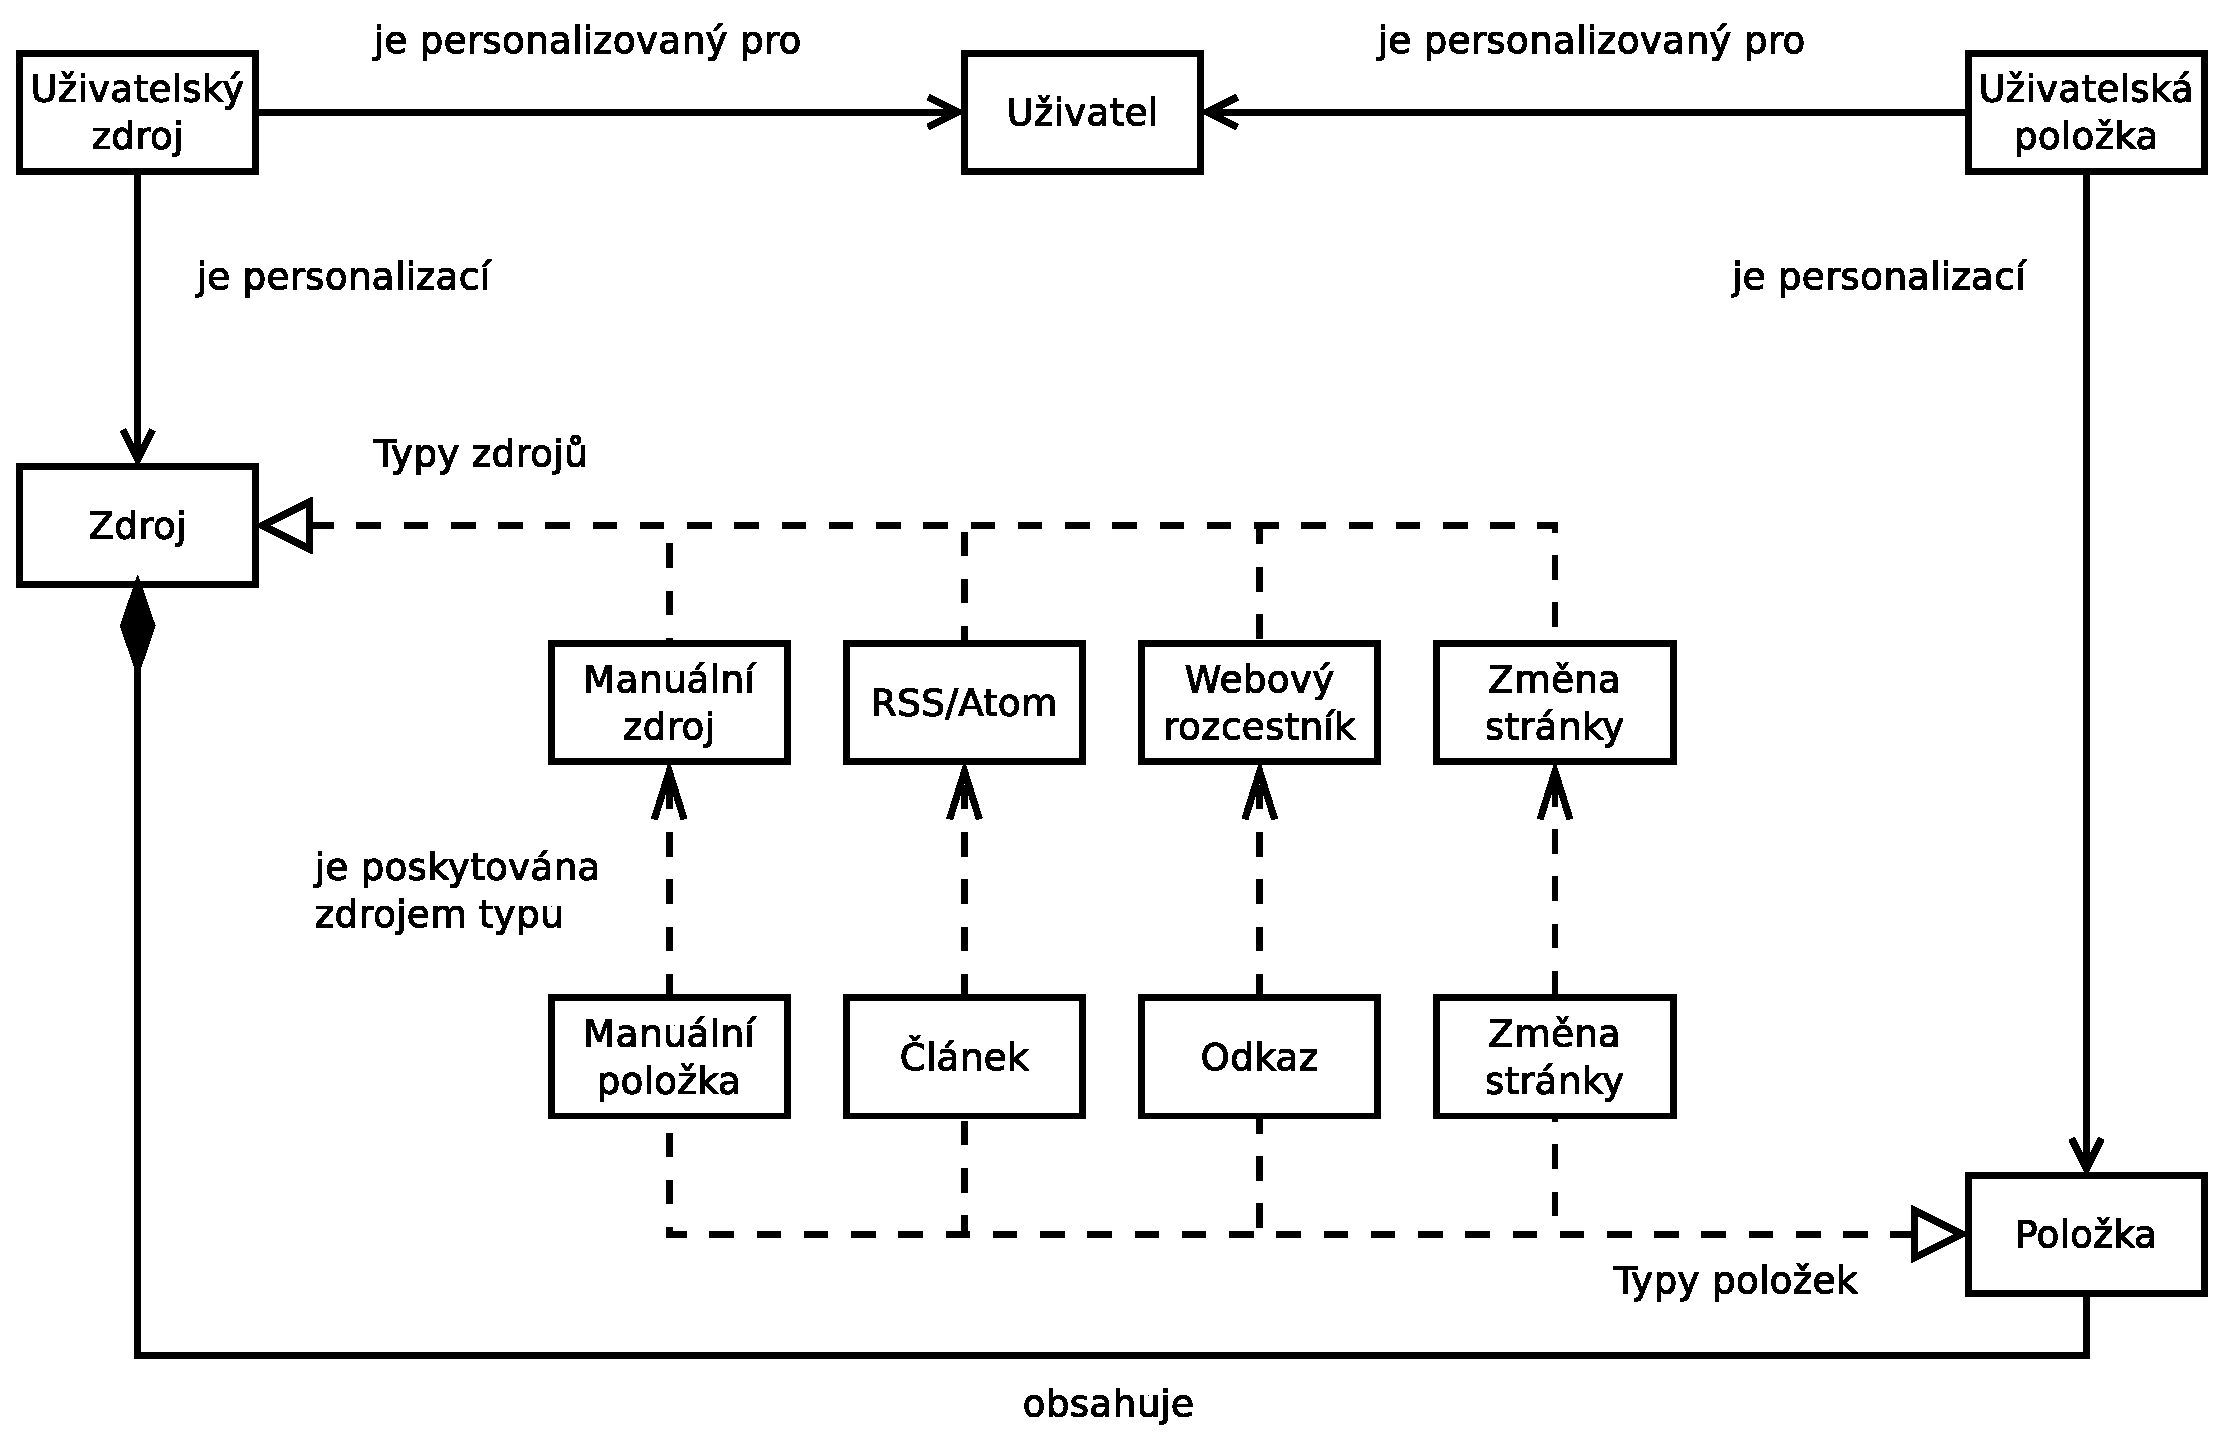
\includegraphics[width=14cm]{zdroje-polozky.eps}
    \caption{Vztahy mezi uživatelem, zdroji a položkami}
    \label{fig:source-item}
\end{figure}

\subsection{Oblast štítků}

Oblast štítků obsahuje entity:

\subsubsection{Seznam položek}
Než zavedeme entity této oblasti, zadefinujeme pojem seznam položek.

Seznam (uživatelských) položek je podle času vzestupně či sestupně uspořádaný seznam všech uživatelských položek, které vyhovují všem kritériím, které jsou uživatelem na seznam kladeny.
Seznam položek je výsledkem dotazu, neexistuje dokud není dotaz proveden.

Termín seznam položek používáme také pro komponentu grafického prostředí, která zobrazuje uživatelské položky, které jsou součástí seznamu položek, výsledku dotazu.

\subsubsection{Štítek}
\label{sss:stitek}

Štítek reprezentuje informaci, kterou může uživatel přidat ke své uživatelské položce.
Štítek má svého vlastníka, uživatele, který jej vytvořil; tento štítek není dostupný jiným uživatelům.
Štítek má několik úloh:
\begin{itemize}
	\item tvoří poznámku u uživatelské položky,
	\item lze filtrovat uživatelské položky mající přiřazený konkrétní štítek,
	\item přiřazením vhodného štítku k uživatelské položce se provede záloha webové stránky položky.
\end{itemize}

Abychom zajistili jednoduché používání štítků, zavedli jsme následující dvě omezení:
\begin{itemize}
	\item Název štítku nesmí obsahovat bílé znaky a znak \$.
		Bílé znaky na okrajích názvu se oříznou, bílé znaky uvnitř a znak \$ způsobí chybu při vytváření/přiřazování štítku.
		Toto omezení vynucuje výstižná jednoslovná pojmenování štítků.
	\item Název štítku nelze později změnit.
		Toto omezení umožňuje využít název štítku jako část jeho klíče.
\end{itemize}

V aplikaci existují dva typy štítků:
\begin{enumerate}
	\item uživatelský štítek -- štítek, který vytvořil uživatel, je přiřazovaný uživatelem a je zobrazovaný v seznamu položek,
	\item zdrojový štítek -- štítek reprezentující uživatelský zdroj -- tento typ štítku není spravován uživatelem, nemůže jej ani vytvořit ani přiřadit, nezobrazuje se v seznamu položek.
\end{enumerate}

\paragraph{Seznam štítků u uživatelských zdrojů}
Uživatel má možnost u svého uživatelského zdroje uvést seznam štítků, které mají být automaticky přidány ke každé uživatelské položce, která patří danému uživatelskému zdroji.
V případě, že zdroj je typu manuální zdroj, nebudou štítky přidány k uživatelské položce automaticky, ale budou jen uživateli nabídnuty přednostně.

Každý uživatelský zdroj obsahuje právě jeden zdrojový štítek; tento štítek zároveň patří právě jednomu uživatelskému zdroji a je vždy součástí zmíněného seznamu štítků.

Můžeme říct, že existuje dvojí vazba mezi uživatelským zdrojem a jeho uživatelskými položkami:
\begin{enumerate}
	\item přímá vazba uživatelské položky na uživatelský zdroj;
	\item nepřímá vazba přes společný zdrojový štítek.
		Tuto vazbu využijeme dále při popisu entity seznamový filtr.
\end{enumerate}

\subsubsection{Seznamový filtr}

Seznamový filtr popisuje kritéria a způsob řazení seznamu položek.
Řazení je vždy buď sestupně či vzestupně podle času přidání uživatelské položky.
Možná kritéria jsou následujících typů:
\begin{itemize}
	\item přečtená/nepřečtená uživatelská položka,
	\item nejstarší/nejnovější datum přidání uživatelské položky,
	\item filtr tvořený predikáty: \uv{Uživatelská položka $X$ má přiřazený štítek $Y$}
\end{itemize}

Poslední uvedené kritérium je zásadní pro funkčnost celé aplikace a všech seznamů položek:
\begin{itemize}
	\item seznam všech položek -- filtr je prázdný
	\item položky nějakého uživatelského zdroje -- filtr obsahuje štítek patřící uživatelskému zdroji
	\item složitější filtry, například seznam položek ze zdroje $X$ nebo položek obsahující zároveň štítek $a$ a $b$:
		\verb|lsrc$X OR lusr$a AND lusr$b|
\end{itemize}

\paragraph{Typy filtrů}
V rámci aplikace rozlišujeme tři typy seznamových filtrů.
\begin{itemize}
	\item obyčejný seznamový filtr -- seznamový filtr, který si uživatel uložil a kdykoli si může zobrazit seznam položek, které mu vyhovují,
	\item exportovaný seznamový filtr -- chová se shodně jako obyčejný seznamový filtr; umožňuje navíc zobrazit seznam položek jako RSS či Atom dokument komukoli mimo naši aplikaci,
	\item ad-hoc seznamový filtr -- slouží pro okamžitou navigaci mezi různými seznamy položek v aplikaci, není trvale uložený.
		Ad-hoc seznamovým filtrem je například realizován seznam položek zobrazený po kliknutí na libovolný štítek.
\end{itemize}

\subsection{Oblast klávesových zkratek}

V aplikaci existuje jediná entita, která popisuje klávesové zkratky.

\subsubsection{Klávesová zkratka}

Klávesová zkratka definuje chování aplikace, které nastane při stisku klávesy či kláves.
Každý uživatel si může definovat svoji vlastní sadu klávesových zkratek.
Rozlišujeme tři různé typy klávesových zkratek:
\begin{itemize}
	\item zkratky, které přiřazují či odebírají štítky uživatelským položkám.
		Klávesová zkratka má vazbu na štítek, který se má k uživatelské položce přidat, pokud přiřazen není, či odebrat, pokud je již přiřazen.
	\item zkratky, které zobrazují seznam položek.
		Klávesová zkratka má vazbu na seznamový filtr, který se má použít pro zobrazení seznamu položek.
	\item zkratky, které vykonávají jednu z mnoha podporovaných akcí.
		Takovou akcí může být například přechod na následující položku, zrušení aktuálního filtru či zobrazení originální stránky položky.
\end{itemize}

\section{Procesy}

Na tomto místě popíšeme procesy, které manipulují s entitami.
Z popsaných procesů je zřejmé, jak jsou jimi realizovány jednotlivé funkční požadavky na aplikaci.

\subsection{Zdroje}

Entity oblasti zdrojů jsme shrnuli v kapitole \ref{sss:shrnuti-zdroju}.
Po přihlášení si uživatel může vytvořit své vlastní zdroje:
\begin{enumerate}
	\item zjistí se, zda takový zdroj již existuje (URL a typ zdroje),
	\item pokud neexistuje vytvoří se nový zdroj příslušného typu,
	\item vytvoří se uživatelský zdroj, který propojí zdroj s uživatelem.
\end{enumerate}

Uživatel nebude moci vytvořit zdroj typu manuální zdroj; manuální zdroj se vytvoří automaticky při prvním přihlášení.
Při každém přihlášení se zkontroluje, zda existuje; pokud neexistuje, vytvoří se výše uvedeným postupem.

Odstranění zdroje není možné z důvodu, že mohou existovat položky, které jsou na tento zdroj navázané.
Uživatel může zrušit sledování zdroje změnou vlastnosti uživatelského zdroje; sledování zdroje může uživatel obnovit.
Pokud bylo u zdroje zrušeno sledování, nebudou se nadále vytvářet uživatelské položky pro tento uživatelský zdroj.
V případě, že neexistuje aktivní uživatelský zdroj pro zdroj, nebude se provádět jeho kontrola.
K tomu může dojít dvěma způsoby:
\begin{itemize}
	\item buď uživatel zrušil sledování zdroje,
	\item nebo během vytváření uživatelského zdroje byl objeven chybně zadaný údaj.
\end{itemize}

\subsection{Položky}

Aplikace pravidelně provádí kontrolu zdrojů; stáhne z internetu dokument odpovídající adrese zdroje a zpracuje jej.
Pokud se při kontrole zdroje zjistí, že záznam ještě v aplikaci neexistuje, bude vytvořen.
\begin{enumerate}
	\item Vytvoří se položka podle typu zdroje,
	\item zjistí se z databáze seznam všech aktivních uživatelských zdrojů pro daný zdroj,
	\item vytvoří se nová uživatelská položka pro každý aktivní uživatelský zdroj.
\end{enumerate}

Uživatel může do aplikace přidat webovou stránku jako novou položku.
V případě, že uživatel přidává položku manuálně:
\begin{enumerate}
	\item nalezne se uživatelský zdroj odpovídající uživatelovu manuálnímu zdroji,
	\item vytvoří se manuální položka pro manuální zdroj nalezeného uživatelského zdroje,
	\item vytvoří se uživatelská položka pro nalezený uživatelský zdroj.
\end{enumerate}

\subsection{Seznamy položek}

Seznam položek je definován seznamovým filtrem -- několika kritérii, kterým musí každá položka vyhovět.
Ad-hoc seznamový filtr vzniká v aplikaci přirozeně akcemi uživatele, je jím realizován například výpis položek uživatelského zdroje.
Uživatel může zobrazit seznam položek na základě svého ad-hoc seznamového filtru; takový seznamový filtr může dále pojmenovat a uložit.
Uživatel si může zadefinovat libovolné množství vlastních seznamových filtrů, přeneseně i seznamů položek.
Seznamový filtr může dále měnit, případně odstranit.

\subsection{Štítky}

Uživatel má možnost přidat k položce dodatečnou informaci prostřednictvím štítku; přidání štítku může probíhat i polo-automaticky (klávesovou zkratkou) či plně automaticky (uvedením štítku do seznamu automaticky přidávaných štítku v uživatelském zdroji).

Uživatel může na několika místech vybrat štítek ze seznamu existujících štítků, případně vytvořit nový, pokud žádaný štítek ještě neexistuje.
Štítek lze odstranit, za předpokladu, že není nikde v aplikaci použit: položkou, seznamovým filtrem, či klávesovou zkratkou.

Pokud má štítek nastavenou vlastnost zálohování, jeho přiřazení uživatelské položce způsobí zazálohování webové stránky položky:
\begin{enumerate}
	\item stáhne se webová stránka položky,
	\item veškeré relativní odkazy na stránce se nahradí za absolutní,
		% TODO link GCS
	\item uloží se soubor stránky do úložiště pomocí služby Google Cloud Storage a zapíše klíč do uživatelské položky.
\end{enumerate}

\subsection{Klávesové zkratky}

Uživatel si může přiřadit klávesové zkratky k nejběžnějším úkonům.
Klávesovou zkratku vytvoří uvedením klávesy či kombinace kláves, které spustí akci, ke které je klávesová zkratka přidána.
Uživatel může klávesovou zkratku odebrat smazáním kombinace kláves, které ji spouští.

Když je klávesová zkratka definována a uživatel stiskne příslušnou kombinaci kláves, spustí se příslušná akce.
Některé akce mohou být závislé na kontextu, ve kterém se uživatel nachází; takovými zkratkami jsou především klávesové zkratky manipulující s aktuálně vybranou uživatelskou položkou v seznamu položek.

\chapter{Dokumentace}
% TODO dokumentace je prý nudná

V této části práce popíšeme funkci/implementaci nejdůležitějších částí aplikace.
Tento popis je určen programátorům; má za cíl poskytnout dostatečný přehled o všech částech aplikace před tím, než se setká se zdrojovým kódem.

\section{Členění aplikace}

Jak jsme již popsali v předchozích kapitolách, aplikace se člení na tři hlavní části:
\begin{enumerate}
	\item serverovou část,
	\item klientskou část,
	\item nepovinný doplněk do prohlížeče.
\end{enumerate}

\begin{figure}
    \centering
    \includegraphics[width=12cm]{cleneni.eps}
    \caption{Vztahy mezi zdrojovým kódem a výsledným produktem kompilace}
    \label{fig:cleneni}
\end{figure}

První dvě části jsou naprogramovány v jazyku Java a sdílejí některé části kódu -- balík \verb|cz.artique.shared|.
Na obrázku~\ref{fig:cleneni} jsou zobrazeny jednotlivé balíky, postup kompilace a její výsledný produkt.

Serverová část závisí na všech balících; můžeme však říci, že závislost na balíku \verb|cz.artique.client| je slabá a vynucená pouze použitým frameworkem GWT.
Vyžaduje, aby rozhraní služby a jeho asynchronní varianta byly ve stejném balíku.
Samotná rozhraní jsou sice implementována jen v balíku \verb|cz.artique.server|, nicméně je nutné je mít přístupné v klientské části.

Sdílená část zdrojového kódu obsahuje především definici modelu -- tříd reprezentujících strukturu dat v databázi podle návrhu entit.
Jednotlivým entitám odpovídá jedna nebo více tříd.

Kromě modelu obsahuje sdílená část rozhraní implementovaná třídami modelu a pomocné třídy používané při komunikaci mezi serverovou a klientskou částí.

\bigskip

Doplněk do prohlížeče je vytvořen zcela odděleně od zbytku aplikace v jazyku JavaScript.

\section{Rozhraní serverové části}

Serverová část je zodpovědná za abstrakci přístupu k databázi, poskytování služeb klientům a vykonávání periodických procesů.

\subsection{Obsluha databáze}
Jelikož platformou poskytovaná databáze neumožňuje složitější operace, navrhli jsme kolekci služeb, které obalují přístup k databázi a provádějí jednoduché manipulace.
Přístup k databázi ze všech částí aplikace směřujeme přes tyto služby.
To nám umožňuje mít přehled o typech prováděných operací a zároveň eliminuje skryté závislosti.
Nejčastějšími operacemi jsou:
\begin{itemize}
	\item získání dalšího objektu podle klíče, například k uživatelskému zdroji doplní region,
	\item získání objektu, příp. jeho vytvoření, pokud neexistuje,
	\item sestavení složitějšího dotazu podle kritérií.
\end{itemize}

\subsection{Rozhraní pro komunikaci s klientskou částí}

Klientská část komunikuje po síti internet se serverovou částí pomocí několika služeb.
Tyto služby lze rozpoznat podle jejich názvu začínajícího slovem \verb|Client|.

\subsubsection{Validace vstupu}

Všechny služby, které jsou veřejně dostupné -- mezi ně patří i služby volané z klientské části -- vždy, bez výjimky, provádějí ošetření hodnot vstupů.
Některé typy validace jsou prováděné z důvodu bezpečnosti, jiné z důvodu zajištění integrity dat či omezení danými použitými knihovnami a databází.
Prováděné úpravy a kontroly hodnot jsou následující:
\begin{itemize}
	\item vyplnění vypočitatelných hodnot; patří sem například:
		\begin{itemize}
			\item výpočet databázového klíče,
			\item dosazení typu z výčtu, pokud existuje jediná možnost,
			\item dosazení aktuálního data do datumových atributů,
			\item nahrazení vlastníka za aktuálně přihlášeného uživatele.
		\end{itemize}
	\item kontrola, zda povinný atribut je vyplněný,
	\item kontrola, zda vlastník všech odkázaných objektů je aktuálně přihlášený uživatel,
	\item oříznutí bílých znaků z řetězců a následná kontrola délky (databáze povoluje řetězce pouze o maximální délce 500 znaků),
	\item oříznutí bílých znaků z delších textů,
	\item kontrola, zda URL je validní,
	\item kontrola, zda URL je validní a webová stránka jí určená je dostupná,
	\item kontrola, zda CSS selektor je validní,
	\item oříznutí bílých znaků z názvu štítku a kontrola, zda název štítku neobsahuje bílé znaky a znak \$.
\end{itemize}

Pokud nebudeme uvažovat validaci, která samotná často zabírá několik desítek řádků kódu, zjistíme, že mnoho z dále popsaných služeb je triviálních.
Tyto služby většinou spočívají jen v zavolání metody poskytnuté obsluhou databáze a vrácení jejího výsledku.

\bigskip
Dále popíšeme rozhraní všech služeb.

\subsubsection{Přihlášení, odhlášení}

Služba \verb|ClientUserService| poskytuje klientské části informace o aktuálně přihlášeném uživateli pomocí jediné metody -- \verb|login|.
Pokud je uživatel přihlášen, vrací metoda objekt uživatele a internetovou adresu určenou k jeho odhlášení.
Součástí objektu uživatele je i klientský token, který se používá při komunikaci s klientským doplňkem.
Zároveň zkontroluje, jestli existuje manuální zdroj pro daného uživatele: pokud neexistuje (uživatel se přihlásil poprvé), vytvoří se.
Naopak, pokud není uživatel přihlášen, vrací jen adresu určenou k přihlášení.

Informaci o aktuálně přihlášeném uživateli přebíráme ze služby \verb|UserService|, kterou nám poskytuje platforma Google AppEngine.

\subsubsection{Kontrola spojení}

Služba \verb|ClientPingService| nemá při běžném chodu aplikace žádný význam, ten získá až v okamžiku, kdy dojde k chybě.
Jakákoli služba pro komunikaci mezi klientskou a serverovou částí může selhat z nejrůznějších důvodů; jedním z důvodů je vypršení času určeného k vyčkání na odpověď.
Pokud dojde k výjimce \verb|RequestTimeoutException|, zkusí se, zda je serverová část vůbec dostupná pomocí metody \verb|ping| této služby.
Její implementace je záměrně triviální z důvodu vyloučení jiných možných chyb.

\subsubsection{Konfigurace}

Služba \verb|ClientConfigService| poskytuje klientské části metody pro získání seznamu všech konfiguračních položek pro aktuálního uživatele.
V případě, že konfigurační položka v databázi neexistuje, vrátí se klientovi s výchozí hodnotou.

Dále tato služba umožňuje dávkovou aktualizaci hodnot několik konfiguračních položek.
Novou hodnotu konfigurační položky uloží služba do databáze pro aktuálně přihlášeného uživatele.

Tato služba v současné době není plně využívána; navrhli jsme ji obecněji, abych si zajistili možnost pozdějšího rozšíření aplikace.

\subsubsection{Zdroje}

Veškeré manipulace jak se zdroji, tak i s uživatelskými zdroji probíhají přes službu \verb|ClientSourceService|.
Zvolili jsme integraci manipulace s několika entitami do jediné služby z důvodu, že klientská část nepracuje se zdroji téměř nikdy přímo, ale výhradně prostřednictvím uživatelských zdrojů.
Tato služba poskytuje následující metody:
\begin{itemize}
	\item přidat zdroj -- vytvoří v databázi zdroj daného typu, pokud ještě neexistoval a vrátí jej.
		Tato metoda se volá v situaci, kdy uživatel vytváří svůj nový uživatelský zdroj: při vytváření uživatelského zdroje je nutná znalost zdroje, který je personalizován.
	\item přidat uživatelský zdroj -- vytvoří v databázi uživatelský zdroj, který je personalizací existujícího zdroje.
		Tato metoda se volá při vytváření uživatelského zdroje po metodě přidat zdroj.
	\item aktualizovat uživatelský zdroj -- aktualizuje v databázi existující uživatelský zdroj.
	\item získat regiony -- vrátí seznam existujících regionů ke zdroji; zdroj musí být typu, který podporuje regiony.
		Tato metoda se volá v okamžiku načtení detailu uživatelského zdroje: buď po jeho vytvoření, nebo během jeho úpravy.
	\item zkontrolovat region -- zkontroluje, zda region je platný.
		Tato metoda může být volitelně zavolána před aktualizací uživatelského zdroje; stejná kontrola se provádí během samotné aktualizace.
	\item naplánovat kontrolu zdroje -- naplánuje okamžitou kontrolu zdroje.
		Mezi naplánováním a spuštěním kontroly může uběhnout časový interval definovaný frekvencí periodické kontroly zdrojů.
		Tato metoda je určena uživatelům pro případ, že se dozví jiným způsobem, že existují nové položky na zdroji dříve, než proběhne jeho řádná naplánovaná kontrola.
	\item získat doporučení -- vrátí předpočítaný seznam doporučených zdrojů pro aktuálního uživatele.
		V situaci, kdy uživatel vytváří nový zdroj, si může vybrat, zda přidá zdroj podle URL adresy či si vybere některý z jemu doporučených.
\end{itemize}

\subsubsection{Štítky}

Veškeré manipulace se štítky probíhají pomocí služby \verb|ClientLabelService|.
Jelikož jsme zavedli silná omezení na štítky, je tato služba spíše jednodušší:
\begin{itemize}
	\item získat všechny štítky -- vrátí všechny štítky z databáze, které patří aktuálně přihlášenému uživateli, bez ohledu na jejich typ.
	\item přidat štítek -- vytvoří nový štítek v databázi, pokud štítek se stejným názvem ještě neexistuje a vrátí jej.
		Tuto metodu volá klientská část v situacích, kdy uživatel má možnost vybrat štítek a uživatel zadá název neexistujícího štítku.
	\item aktualizovat štítky -- provede dávkovou aktualizaci v databázi několika štítků; nastavením atributu \verb|toBeDeleted| lze štítek odstranit.
		Odstranění štítku je podmíněné tím, že není nikde použitý; v opačném případě odstranění selže.
\end{itemize}

\subsubsection{Seznamové filtry}

Služba \verb|ClientListFilterService| provádí veškeré manipulace se seznamovými filtry.
Nabízí obvyklé metody:
\begin{itemize}
	\item získat všechny seznamové filtry -- vrátí z databáze seznam všech seznamových filtrů, které patří aktuálně přihlášenému uživateli.
	\item přidat seznamový filtr -- uloží seznamový filtr do databáze.
	\item aktualizovat seznamový filtr -- aktualizuje v databázi seznamový filtr.
	\item odstranit seznamový filtr -- odstraní z databáze seznamový filtr.
\end{itemize}

\subsubsection{Položky}

Nejkomplexnější a nejdůležitější službou, kterou serverová část poskytuje klientské části je \verb|ClientItemsService|.
Tato služba poskytuje 3 metody, které manipulují s položkami:
\begin{itemize}
	\item Přidat manuální položku -- vytvoří v databázi novou manuální položku a odpovídající uživatelskou položku k manuálnímu zdroji aktuálně přihlášeného uživatele.
	\item Získat položky -- vrátí seznam uživatelských položek, které vyhovují seznamovému filtru.
		Pokud nejde o první dotaz, bude v dotazu uvedený i klíč poslední uživatelské položky, kterou klientská část zná; vráceny budou jen novější/starší uživatelské položky (závisí na způsobu řazení).
		V případě, že seznam má být řazený sestupně, bude výsledek obsahovat i seznam uživatelských položek, které jsou novější než klientské části známá nejnovější uživatelská položka.
		Výsledek obsahuje i informaci o tom, zda mohou existovat ještě další uživatelské položky -- jestli existuje šance, že následující dotaz vrátí neprázdný výsledek.
	\item Aktualizovat položky -- aktualizuje v databázi uživatelské položky na základě souboru změn, které se na ně mají aplikovat.
		Soubor změn udává, které štítky se mají uživatelské položce přidat či odebrat a jaký má být její nový stav (přečtená -- nepřečtená).
		Metoda vrací seznam uživatelských položek, které byly změněny.
\end{itemize}

\subsubsection{Klávesové zkratky}

Klávesová zkratka je jednoduchá entita, na níž není kladen požadavek složitější manipulace; vystačíme si s možností vytvoření a odstranění klávesové zkratky.
Tato služba poskytuje následující metody:
\begin{itemize}
	\item získat všechny klávesové zkratky -- vrátí z databáze seznam všech klávesových zkratek aktuálně přihlášeného uživatele.
	\item vytvořit klávesovou zkratku -- vytvoří v databázi klávesovou zkratku.
	\item odstranit klávesovou zkratku -- odstraní klávesovou zkratku z databáze.
\end{itemize}

Změna klávesové zkratky je možná posloupností odstranění staré zkratky a následného vytvoření nové zkratky.

\subsection{Rozhraní pro komunikaci s klientským doplňkem}

Služba pro komunikaci s klientským doplňkem -- \verb|ClientServlet| vyžaduje přihlášení uživatele.
Rozhodli jsme se přidělit každému uživateli náhodný jednoznačný identifikátor, který bude doplněk v prohlížeči používat při komunikovat se serverovou částí aplikace ke své identifikaci.
Tento identifikátor -- token -- je určen jen a pouze pro komunikaci s doplňkem.
Myslíme si, že jde o rozumný kompromis mezi zajištěním bezpečí a jednoduchostí implementace.

Rozhraní pro komunikaci s doplňkem nabízí dvě metody:
\begin{itemize}
	\item získat štítky -- vrátí z databáze seznam názvů všech uživatelských štítků.
		Funguje velice podobně jako metoda získat všechny štítky služby štítků pro komunikaci s klientskou částí.
		Liší se jen tím, že tato metoda filtruje štítky podle typu a vrací ještě seznam výchozích štítků pro manuální zdroj.
	\item přidat položku -- přidá položku popsanou \zkratka{JSON}{JavaScript Object Notation -- textový formát určený pro přenos strukturovaných dat založený na syntaxi jazyku JavaScript} objektem k manuálnímu zdroji uživatele.
		Provádí podobné kontroly a úpravy jako metoda přidat manuální položky služby položek pro komunikaci s klientskou částí.
		Jelikož toto rozhraní je textové (nepřenáší se klíče štítků, ale jejich názvy), může uživatel přidělit položce i neexistující štítek.
		V takovém případě bude v okamžiku, kdy je zřejmé, že objekt položky prošel všemi kontrolami, vytvořen nový štítek a následně k uživatelské položce přiřazen.
\end{itemize}

Při použití tohoto klientského rozhraní musí klient poskytnout svůj klientský token a uvést akci (metodu), která se má provést.

\subsection{Rozhraní pro plánování a plánované úlohy}

Do této skupiny jsme zařadili služby, které jsou spouštěny:
\begin{itemize}
	\item buď periodicky plánovačem \pojem{Cron}{plánovač, který spouští úlohy periodicky v předem určený čas} (kontrola zdrojů, výpočet doporučení),
	\item nebo jsou realizovány pomocí úloh, které se postupně zpracovávají (kontrola zdrojů, zálohování položky)
\end{itemize}

\subsubsection{Kontrola zdrojů}

Naše aplikace vyžaduje pro získávání nového obsahu periodické spouštění kontroly zdrojů.
Cronem spouštěná služba nejprve zjistí seznam zdrojů, které je třeba zkontrolovat: to jsou takové, jejichž plánovaný čas kontroly je menší než aktuální čas, nenastalo u nich příliš mnoho chyb během poslední kontroly a zároveň nejsou právě kontrolovány.
Pro každý nalezený zdroj se vytvoří úloha, která je následně vložena do fronty.
Fronta úloh se stará o to, aby byly jednotlivé úlohy spouštěny postupně s určitou frekvencí, což snižuje okamžitou zátěž.
Dalšími výhodami naplánování úloh oproti okamžitému spuštění kontroly zdroje jsou:
\begin{itemize}
	\item možnost kontroly několika zdrojů zároveň -- každá kontrola probíhá ve vlastním vlákně,
	\item maximální doba běhu skriptu se týká každé kontroly zvlášť, nehrozí tak vypršení časového limitu.
	\item možnost opakování kontroly zdroje v případě, že dojde k chybě.
\end{itemize}

Aby se aplikace lépe vypořádala s chybnými zdroji (nekontrolovala je nepřiměřeně často), po několika chybách při kontrole zastavíme jeho další kontroly v normálním režimu.
Takový zdroj bude kontrolován v chybovém režimu, méně často, jen jednou za 12 hodin; v případě, že se následná kontrola zdaří, vrátí se zdroj do normálního režimu.

\subsubsection{Výpočet doporučení}

Seznam zdrojů doporučovaných jednotlivým uživatelům přepočítáváme z důvodů, které jsme zmínili v kapitole~\ref{sec:volba-systemu-doporucovani}, jen jednou za den.
O pravidelné spouštění procesu se stará Cron poskytovaný platformou Google AppEngine.

Výpočet probíhá v několika krocích:
\begin{enumerate}
	\item Načtení všech uživatelských zdrojů z databáze a vytvoření matice uživatelů a zdrojů.
		Matice má v řádcích uživatele, ve sloupcích zdroje.
		Prvek matice vyplníme:
		\begin{itemize}
			\item buď jedničkou, pokud existuje uživatelský zdroj – uživatel sleduje zdroj,
			\item nebo nulou v opačném případě.
		\end{itemize}
		Tvorbou matice z uživatelských zdrojů si zajistíme přítomnost alespoň jedné jedničky v každém řádku i sloupci.
		Matici nazveme $M$.
	\item Matici normalizujeme zvlášť v řádcích a sloupcích: každý řádek, resp. sloupec vydělíme jeho součtem.
		Tato normalizace nám zajistí rovnost vah všech uživatelů, resp. zdrojů (jinak by měl větší váhu uživatel s mnoha zdroji resp. zdroj sledovaný mnoha uživateli).
		Matici s normalizovanými zdroji pro uživatele nazveme $M_u$.
		Matici s normalizovanými uživateli pro zdroje nazveme $M_z$
	\item Připravíme si čtvercovou matici popisující vhodnost uživatelů: jak jsou si uživatelé blízcí.
		Před začátkem výpočtu je tato matice jednotková; zatím neznáme blízké uživatele (reflexivita zajišťuje stabilitu výpočtu).
		Matici označíme $U_0$; $U = U_0$ bude matice používaná během výpočtu.
	\item Provedeme krok výpočtu:
		aktualizujeme nejprve váhy zdrojům pro všechny uživatele:
			$ Z = U \cdot M_u $
		a následně aktualizujeme blízkost každých dvou uživatelů:
			$ U = Z \cdot M_z + U_0 $.
	\item Několikrát provedeme iteraci 4. kroku výpočtu.
	\item Matice $Z$ obsahuje váhy popisující vhodnost zdroje pro každého uživatele.
		Matici budeme procházet po řádcích (pro uživatele); setřídíme zdroje podle vah sestupně a vyfiltrujeme ty, které uživatel již sleduje (jsou v matici $M$).
		Ze seznamu vezmeme prvních $k$ doporučených zdrojů a výsledný seznam uložíme pro každého uživatele do databáze.
\end{enumerate}

\subsubsection{Zálohování položky}

Kdykoli je nějaké uživatelské položce přiřazen štítek, zkontroluje se, zda štítek má nastavenou vlastnost zálohování.
Pokud ji má, vytvoří se nová zálohovací úloha, která se zařadí do fronty.
Stejně jako v případě kontroly zdrojů, i zde se fronta úloh stará o jejich postupné spouštění.
Postup zálohování jsme popsali v části~\ref{ssec:procesy-stitky} 

\subsection{Veřejné rozhraní k obsahu}

Některá rozhraní aplikace jsou dostupná i neregistrovaným uživatelům

\subsubsection{Exportování položek}

Toto rozhraní poskytuje seznam položek vyhovujících seznamovému filtru, u kterého jeho vlastník povolil možnost exportování.
Export je identifikovaný kombinací aliasu a uživatelského jména vlastníka seznamového filtru.
Služba zodpovědná za výběr položek z databáze je stejná jako v případě poskytování seznamu položek klientské položky se všemi svými důsledky.
Seznam položek je vrácen buď ve formě RSS, nebo Atom (záleží na parametru poskytnutého v URL).

\subsubsection{Zálohované položky}

Připomeňme, že během zálohování stáhneme webovou stránku, mírně ji upravíme a uložíme; záloze je přidělen klíč, který ji identifikuje.
Odkaz na zálohovanou stránku (přístupnou přes toto rozhraní) je dostupný uživateli, který zálohu provedl ze seznamu položek.

\section{Členění klientské části}

Doposud jsme se příliš klientskou části nezabývali z důvodu, že klientská část přímo neprovádí žádné manipulace s daty; využívá pouze prostředků, které jí poskytuje serverová část.
Přesto můžeme klientskou část rozčlenit do několika částí (spíše podle funkce než podle balíků):
\begin{itemize}
	\item realizace hierarchií a stromových komponent,
	\item správci, kteří komunikují se serverovou částí a ostatní správci,
	\item komponenta nekonečného seznamu,
	\item dialogy, pomocí kterých se vytvářejí a upravují všechny objekty.
\end{itemize}

\subsection{Hierarchie}
% FIXME lépe popsat hierarchie

Vzhledem ke způsobu uložení hierarchie v databázi: popisujeme cestu ke kořeni, je nutné pro zobrazení stromu primárně vlastní hierarchii vybudovat.
Všichni správci, kteří poskytují hierarchii, musejí každý objekt, který spravují, zpracovat a vložit do uměle vytvořené hierarchie.
Postup vypadá následovně:
\begin{enumerate}
	\item Vytvoření kořenového uzlu.
	\item Pro všechny spravované objekty:
	\item rozdělení cesty ke kořeni podle lomítek (oddělovačů jednotlivých úrovní),
	\item vytvoření uzlů pro jednotlivé úrovně, pokud ještě neexistují,
	\item vytvoření listu v nejnižší úrovni; jeho hodnotou bude příslušný objekt.
	\item Vrácení kořenového uzlu.
\end{enumerate}

Uzly se stejným rodičem jsou řazeny podle abecedy.

Z důvodu propagace změn, všechny uzly umožňují zaregistrování posluchače událostí změn v hierarchii: uzel byl přidán, odebrán, název uzlu se změnil.

\subsubsection{Stromové komponenty}

Klientská část aplikace obsahuje tři komponenty, které umožňují zobrazit hierarchie v podobě stromu; jsou to:
\begin{itemize}
	\item strom zdrojů -- hierarchii poskytuje správce zdrojů,
	\item strom seznamových filtrů -- hierarchii poskytuje správce seznamových filtrů,
	\item strom zpráv -- hierarchii poskytuje správce zpráv.
\end{itemize}

Zprávy ve skutečnosti netvoří strom ale prostý seznam.
Využili jsme stromovou komponentu pro jejich zobrazení z několika důvodů:
\begin{itemize}
	\item poskytuje všechny možnosti, které vyžadujeme,
	\item vzhled seznamu zpráv je blízký vzhledu stromů zdrojů a stromu seznamových filtrů,
	\item zjednodušuje výslednou implementaci.
\end{itemize}

\subsection{Správci}

Téměř každé službě, kterou jsme popsali z pohledu serverové části odpovídá správce v klientské části.
Správce má za úkol zprostředkovávat veškerou komunikaci se serverovou částí a poskytovat nakešovaná data.
Každý správce poskytuje klientské části rozhraní k metodám služby, kterou obaluje.
Tento obal většinou spočívá v zavolání příslušné metody služby a ve většině případů zobrazení zprávy o výsledku.
Hlášku o úspěchu zobrazuje v případě, že volání metody bylo vyvoláno akcí uživatele.
V případě neúspěchu zobrazíme zprávu vždy; ta obsahuje informaci, proč volání selhalo, například z důvodu nevyplnění některého z atributů.
Navíc se zavolá služba kontroly spojení pro zjištění, zda je vůbec dostupné spojení se serverovou částí.

V popisu jednotlivých správců budeme zmiňovat pouze metody, které provádějí netriviální další akce.

\subsubsection{Správce konfigurace}

Správce konfigurace tvoří jen obálku kolem vlastní služby.
V okamžiku spuštění si stáhne veškerou konfiguraci relevantní pro přihlášeného uživatele.
Jednotlivé dotazy na konfigurační položky pak může zodpovídat okamžitě bez nutnosti komunikace se serverovou částí.

Správce konfigurace umožňuje rovněž i aktualizovat hodnoty konfiguračních položek, nicméně tuto možnost naše aplikace v současné době nevyužívá.

\subsubsection{Správce zdrojů}

Správce zdrojů načte ze serveru seznam všech uživatelských zdrojů přihlášeného uživatele.
Jednotlivé uživatelské zdroje uloží do několika slovníků, aby byly rychle vyhledatelné: podle klíče uživatelského zdroje a podle zdrojového štítku.
Ze všech uživatelských zdrojů vybuduje hierarchii.
Správce zdrojů si pamatuje, který zdroj je manuální (vždy existuje právě jeden).

Jelikož správce zdrojů poskytuje přístup k hierarchii uživatelských zdrojů, musí reagovat na určitě události.
Jakékoli úspěšné volání metody přidat uživatelský zdroj či aktualizovat uživatelský zdroj může způsobit změnu hierarchie.
Správce zdrojů ve zmíněných metodách případně upravují hierarchii uživatelských zdrojů.

\subsubsection{Správce štítků}

Správce štítků obsahuje seznam všech štítků rozdělených podle typů: uživatelský štítek, zdrojový štítek, systémový štítek.
Existují dva systémové štítky, oba reprezentují operátory: AND -- operátor \textit{a}, OR -- operátor \textit{nebo}.
Zbylé dva seznamy štítků (uživatelských a zdrojových) jsou naplněny dotazem na serverovou část při prvním spuštění správce.
Každému štítku je nastaven zobrazovaný název: u uživatelských štítků je to jejich vlastní název, u zdrojových je to název zdroje ke kterému štítek patří.

Správce štítků poskytuje metodu pro vyhledávání štítků podle části jejich názvu.
Tuto metodu používá komponenta, která nabízí štítky v situaci, kdy uživatel může vložit název štítku (například, pokud se přidává štítek uživatelské položce).

V případě, že uživatel přidá novou položku doplňkem v prohlížeči a přiřadí ji dosud neexistující štítek, dostane se klientská část do zvláštní situace.
Seznam uživatelských položek by měl obsahovat uživatelskou položku se štítkem, o kterém nemá žádnou informaci.
Samotná uživatelská položka zná pouze klíč štítku a správce štítků by jí měl objekt štítku dodat.
V takovém případě se aktualizace seznamu položek pozastaví a bude pokračovat, až si správce štítků obnoví seznam všech existujících štítků dotazem na serverovou část.

\subsubsection{Správce seznamových filtrů}

Správce seznamových filtrů poskytuje hierarchii všech seznamových filtrů, kterou si vytvoří po svém spuštění.
Dále poskytuje metody pro manipulaci se seznamovými filtry, které v případě úspěchu upraví hierarchii.
Těmito metody jsou: přidat seznamový filtr, aktualizovat seznamový filtr a odstranit seznamový filtr.

\subsubsection{Správce položek}

Správce položek poskytuje transparentní rozhraní k metodám: získat položky a přidat manuální položku.
Poslední metoda příslušné služby -- aktualizovat položky -- není uživateli přímo dostupná.

Správce položek si udržuje seznam změn jednotlivých uživatelských položek, které se mají provést v databázi na straně serveru.
Uživatel tento seznam změn vytváří a upravuje metodami:
\begin{itemize}
	\item štítek přidán -- přidá štítek (jeho klíč) do seznamu štítků k přidání v sadě změn příslušející uživatelské položce,
	\item štítek odebrán -- přidá štítek (jeho klíč) do seznamu štítků k odebrání v sadě změn příslušející uživatelské položce,
	\item přečtena -- nastaví stav přečtení v sadě změn příslušející uživatelské položce.
\end{itemize}

Změna v grafickém rozhraní se provede okamžitě, odeslání změny na server se odloží.
V případě posloupnosti přidání a odebrání stejného štítku od uživatelské položky se obě změny vyruší.
Periodicky, každých několik sekund probíhá dotaz obsahující seznam všech sad změn mezi správcem položek a službou serverové části.
Toto \uv{zpoždění} provedení změny v databázi nám umožňuje snížit počet dotazů po síti a zvýšit subjektivní rychlost odezvy aplikace.

\subsubsection{Správce klávesových zkratek}

Správce klávesových zkratek si při svém spuštění načte pomocí serverové služby seznam všech klávesových zkratek, které si uživatel sám definoval.
Kombinace kláves klávesových zkratek rozparsuje a klávesové zkratky vloží do slovníku.
Dále zaregistruje posluchače událostí stisknutí klávesy: události \verb|KeyPress| a \verb|KeyDown|.
Pokud je detekováno stisknutí kláves odpovídající nějaké zkratce, vyvolá správce událost \verb|ShortcutEvent|, pomocí které informuje o klávesové zkratce své posluchače.
Sám správce klávesových zkratek zpracovává některé obecné typy zkratek: navigace mezi seznamy položek, jejich obnovu a podobné.

Správce poskytuje metody vytvořit klávesovou zkratku a odstranit klávesovou zkratku.
Tyto metody v případě úspěchu upraví slovník klávesových zkratek.

Některé typy klávesových zkratek se odkazují na jiné objekty (štítky a seznamové filtry).
Tyto klávesové zkratky je možné vyhledat na základě klíče objektu, na který se odkazují.
Využíváme toho v dialozích s nastavením seznamových filtrů a dialogu s nastavením štítků.

\bigskip

Zbylí dva správci nejsou závislí na službách serverové části; spravují objekty, které mají význam pouze v kontextu klientské části.

\subsubsection{Správce zpráv}

Zpráva je krátký text o různé důležitosti, který slouží k informování uživatele o úspěchu či selhání některé akce.

Správce zpráv je centrálním bodem v naší aplikaci pro zpracování zpráv.
Poskytuje rozhraní klientské části aplikace, přes které může kterákoli komponenta zobrazit zprávu.
Správce zpráv také poskytuje seznam posledních zpráv v podobě hierarchie.

Správce sám zprávy nezobrazuje, ale umožňuje zaregistrovat posluchače, kteří mají být zpraveni o nových zprávách.
Jediným posluchačem je vlastní grafická komponenta zodpovědná za zobrazování zpráv.


\subsubsection{Správce historie}

Framework GWT obsahuje podporu pro sledování historie v rámci aplikace.
Jednou položkou v historii je token -- řetězec reprezentující aktuální stav aplikace.
V našem případě stav aplikace odpovídá zobrazenému seznamovému filtru.

Náš správce historie rozšiřuje tento mechanismus o několik důležitých vlastností.
Pro nás je užitečnější znalost samotného seznamového filtr než jeho serializované varianty; z toho důvodu si ukládáme do seznamu stavů dvojici token -- seznamový filtr a nižší vrstvě (GWT) předáváme token.
Při reakci na událost změna historie, kterou vyvolá GWT reagujeme změnou aktuálního seznamového filtru a vyvoláním vlastní událost \verb|HistoryEvent|, pomocí které informujeme příslušnou část aplikace o změně.

\subsection{Nekonečný seznam}

V této části pod pojmem položka myslíme jeden záznam v seznamu, který je reprezentován uživatelskou položkou.

Nejdůležitější grafickou komponentou, která tvoří naši aplikaci, je nekonečný seznam položek.
Nazýváme ho nekonečným, neboť nemá konec – jakmile uživatel odroluje seznam ke konci, načtou se další položky; takto jich může postupně zobrazit stovky.
Samozřejmě, že v případě omezeného množství položek, vlastní konec seznamu existuje, avšak může být prakticky nedosažitelný.
Výhodou tohoto přístupu je možnost stahovat ze serverové části pouze data, o která má uživatel právě zájem.

Položky, které jsou v seznamu zobrazené, jsou dodávané poskytovatelem, který reaguje na událost odrolování blízko konce seznamu zavoláním metody získat položky správce položek.
Kdykoli se změní aktuální seznamový filtr, zruší se původní poskytovatel a nahradí se novým.

Nekonečný seznam je posluchačem událostí \verb|ShortcutEvent| správce zkratek; reaguje na zkratky typu: přesun na předchozí/další položku, zobrazit originální webovou stránku, přidat/odebrat štítek a podobné.

Každý řádek reprezentuje jednu uživatelskou položku se všemi jejími informacemi: zdroj ze kterého pochází, datum a čas přidání položky, seznam přiřazených štítků a hlavně titulek.
Obsah položky (text nebo HTML) se zobrazí pouze v případě, že položka je vybraná a rozbalená.

\subsection{Dialogy}
Manipulace s daty v aplikaci probíhá v rámci dvou oblastí: v nekonečném seznamu a přes dialogy.
V nekonečném seznamu může uživatel provádět následující operace:
\begin{itemize}
	\item označení uživatelské položky jako přečtené,
	\item přidání/odebrání štítku uživatelské položce, příp. vytvoření nového štítku, pokud zadá neexistující název.
\end{itemize}

Všechny ostatní operace provádí uživatel prostřednictvím dialogů -- oken, která dočasně překryjí stránku aplikace.
Každá oblast, kterou jsme dříve zmínili, s výjimkou položek a konfigurace, nabízí jeden či více dialogů pro svoji konfiguraci:
\begin{itemize}
	\item vytvoření a úpravu zdroje,
	\item vložení manuální položky,
	\item vytvoření a úpravu seznamového filtru, úpravu ad-hoc seznamového filtru,
	\item úpravu a odstranění klávesových zkratek,
	\item tvorbu klávesové zkratky typu akce,
	\item úpravu a odstranění štítku.
\end{itemize}

Každý z těchto dialogů má jinou grafickou podobu závislou na atributech spravované třídy.
V případě, že uživatel změnu provedenou v dialogu potvrdí, zavolají se metody příslušných správců, které změnu delegují na služby serverové části.

\section{Doplněk do prohlížečů}

Doplněk do prohlížeče je nepovinné rozšíření aplikace, které má za cíl zjednodušit její ovládání uživatelům.
Implementace doplňku spoléhá na API poskytované platformou Crossrider, na níž je postaven.
Doplněk můžeme rozdělit do tří částí, které spolu komunikují; pro jednoduchost je budeme pojmenovávat terminologií platformy:
\begin{itemize}
	\item background -- skript, který běží v prohlížeči na pozadí; je nezávislý na otevřených stránkách; existuje vždy v jediné instanci,
	\item extension -- skript, který se vykonává zvlášť v rámci každé otevřené stránky
	\item popup -- html stránka, která se zobrazí při kliknutí na ikonku doplňku v liště prohlížeče; mezi dvěma zobrazeními se stav nezachovává.
\end{itemize}

\begin{figure}
	\centering
	\includegraphics[width=9cm]{doplnek-init.eps}
	\caption{Postup inicializace doplňku}
	\label{fig:doplnek-init}
\end{figure}
\begin{figure}
	\centering
	\includegraphics[width=11cm]{doplnek-akce.eps}
	\caption{Postup zobrazení popupu a vytvoření manuální položky}
	\label{fig:doplnek-akce}
\end{figure}

\subsection{Inicializace doplňku}

Doplněk se inicializuje při spuštění prohlížeče vykonáním background skriptu; postup je znázorněn na obrázku~\ref{fig:doplnek-init}.
Nejprve zkontrolujeme, zda známe klientský token (1, 2); pokud ho známe, nastavíme akci zobrazení popup stránky při kliknutí na ikonku (3).
V případě, že token neznáme, budeme čekat na zprávu o dostupnosti tokenu (1', 2').
Až token budeme znát, nastavíme popup stránku (kroky 1, 2, 3).

Skript extension zjišťuje podle URL adresy aktuální stránku; pokud se jedná o stránku naší aplikace, vyhledá v hlavičce stránky elementu meta s názvem \verb|clientToken|.
Tento meta element do stránky přidá klientská část aplikace při své inicializaci.

\subsection{Přidání manuální položky}

Postup je znázorněn na obrázku~\ref{fig:doplnek-akce}.
Uživatel vyvolá akci vložení aktuální stránky do naší aplikace kliknutím na ikonu doplňku v liště prohlížeče (1).
Zobrazí se vyskakovací (popup) okno s formulářem, který bude předvyplněný informacemi o aktuální stránce: titulek, URL, vybraná část textu.
Informace se získají zasláním zprávy (6) skriptu běžícímu v aktuálně otevřené stránce; skript zašle zpět (7) požadované údaje.

Formulář bude dále obsahovat předvyplněný seznam štítků a umožní přidat další štítky.
Popup zašle zprávu (2) background skriptu, který odešle dotaz (3) na serverovou část pomocí metody \verb|post| poskytované platformou Crossrider.
Background skript odpověď (4) zašle zpět (5) do popup okna.

Pokud uživatel odešle formulář, odchytí skript událost odeslání a zašle background skriptu zprávu (8) s vyplněnými údaji o manuální položce, kterou chce uživatel přidat.
Background skript odešle dotaz (9) serverové části pomocí metody \verb|post|.
Využití této metody je nutné z důvodu obejití některých omezení prohlížeče: skript může kontaktovat jen stránky ze stejné domény.

\chaptert{Závěr}

Výsledkem naší práce na tomto projektu je aplikace, která je, dle našeho názoru, schopná nabídnout uživatelům vlastnosti, které se od čtečky očekávají.
Aplikace v sobě navíc kombinuje několik dalších služeb, díky nimž je unikátní; nejedná se \uv{jen o další čtečku}.
Z tohoto pohledu považujeme náš cíl za splněný.

Čtečku jsme navrhli a vytvořili především tak, aby odpovídala našim požadavkům.
Aplikace nabízí následující možnosti:
\begin{itemize}
	\item sledovat libovolný kanál RSS nebo Atom,
	\item získávat informace o změnách i ze stránek, které zmíněné kanály neposkytují,
	\item doporučovat zdroje, které sledují podobní uživatele,
	\item přidat vlastní internetovou adresu jako novou položku (použitím rozhraní aplikace nebo prostřednictvím volitelného doplňku),
	\item přiřadit položkám štítky,
	\item filtrovat položky podle zdrojů či štítků,
	\item ukládat své filtry a používat je jako seznamy položek,
	\item zálohovat aktualní stav webové stránky reprezentované položkou,
	\item exportovat seznam položek jako RSS nebo Atom kanál,
	\item ovládat většinu aplikace jen pomocí konfigurovatelných klávesových zkratek.
\end{itemize}

Podařilo se nám vyhovět všem důležitým požadavkům, a tím i vyřešit identifikované nevýhody jiných čteček.
Věříme proto, že aplikace má potenciál být využívána.


%%% Seznam použité literatury je zpracován podle platných standardů. Povinnou citační
%%% normou pro bakalářskou práci je ISO 690. Jména časopisů lze uvádět zkráceně, ale jen
%%% v kodifikované podobě. Všechny použité zdroje a prameny musí být řádně citovány.

%\def\refname{Použitá literatura a prameny}
\def\bibname{Seznam použité literatury}
\bibliographystyle{czechiso}
\bibliography{literatura}

%\begin{thebibliography}{99}
%\addcontentsline{toc}{chapter}{\bibname}

%\bibitem{lamport94}
%  {\sc Lamport,} Leslie.
%  \emph{\LaTeX: A Document Preparation System}.
%  2. vydání.
%  Massachusetts: Addison Wesley, 1994.
%  ISBN 0-201-52983-1.

%\end{thebibliography}

%\chapwithtoc{Seznam použitých zkratek}
\renewcommand{\nomname}{Seznam použitých zkratek}
\renewcommand{\nomlabel}[1]{\textbf{#1}}
\printnomenclature

\end{document}
